\documentclass[a4paper]{article}

\usepackage[pdftex,
  hidelinks,
  pdfauthor={Dexter Chua},
  pdfsubject={Cambridge Maths Notes: Part IA - Dynamics and Relativity},
  pdftitle={Part IA - Dynamics and Relativity},
pdfkeywords={Cambridge Mathematics Maths Math IA Lent Dynamics and Relativity}]{hyperref}

\title{Part IA - Dynamics and Relativity}
\author{Lectured by G. I. Ogilvie}
\date{Lent 2015}

% Imports
\ifx \nextra \undefined
  \usepackage[pdftex,
    hidelinks,
    pdfauthor={Dexter Chua},
    pdfsubject={Cambridge Maths Notes: Part \npart\ - \ncourse},
    pdftitle={Part \npart\ - \ncourse},
  pdfkeywords={Cambridge Mathematics Maths Math \npart\ \nterm\ \nyear\ \ncourse}]{hyperref}
  \title{Part \npart\ - \ncourse}
\else
  \usepackage[pdftex,
    hidelinks,
    pdfauthor={Dexter Chua},
    pdfsubject={Cambridge Maths Notes: Part \npart\ - \ncourse\ (\nextra)},
    pdftitle={Part \npart\ - \ncourse\ (\nextra)},
  pdfkeywords={Cambridge Mathematics Maths Math \npart\ \nterm\ \nyear\ \ncourse\ \nextra}]{hyperref}

  \title{Part \npart\ - \ncourse \\ {\Large \nextra}}
\fi

\author{Lectured by \nlecturer \\\small Notes taken by Dexter Chua}
\date{\nterm\ \nyear}

\usepackage{alltt}
\usepackage{amsfonts}
\usepackage{amsmath}
\usepackage{amssymb}
\usepackage{amsthm}
\usepackage{booktabs}
\usepackage{caption}
\usepackage{enumitem}
\usepackage{fancyhdr}
\usepackage{graphicx}
\usepackage{mathtools}
\usepackage{microtype}
\usepackage{multirow}
\usepackage{pdflscape}
\usepackage{pgfplots}
\usepackage{siunitx}
\usepackage{tabularx}
\usepackage{tikz}
\usepackage{tkz-euclide}
\usepackage[normalem]{ulem}
\usepackage[all]{xy}

\pgfplotsset{compat=1.12}

\pagestyle{fancyplain}
\lhead{\emph{\nouppercase{\leftmark}}}
\ifx \nextra \undefined
  \rhead{
    \ifnum\thepage=1
    \else
      \npart\ \ncourse
    \fi}
\else
  \rhead{
    \ifnum\thepage=1
    \else
      \npart\ \ncourse\ (\nextra)
    \fi}
\fi
\usetikzlibrary{arrows}
\usetikzlibrary{decorations.markings}
\usetikzlibrary{decorations.pathmorphing}
\usetikzlibrary{positioning}
\usetikzlibrary{fadings}
\usetikzlibrary{intersections}
\usetikzlibrary{cd}

\newcommand*{\Cdot}{\raisebox{-0.25ex}{\scalebox{1.5}{$\cdot$}}}
\newcommand {\pd}[2][ ]{
  \ifx #1 { }
    \frac{\partial}{\partial #2}
  \else
    \frac{\partial^{#1}}{\partial #2^{#1}}
  \fi
}

% Theorems
\theoremstyle{definition}
\newtheorem*{aim}{Aim}
\newtheorem*{axiom}{Axiom}
\newtheorem*{claim}{Claim}
\newtheorem*{cor}{Corollary}
\newtheorem*{defi}{Definition}
\newtheorem*{eg}{Example}
\newtheorem*{fact}{Fact}
\newtheorem*{law}{Law}
\newtheorem*{lemma}{Lemma}
\newtheorem*{notation}{Notation}
\newtheorem*{prop}{Proposition}
\newtheorem*{thm}{Theorem}

\renewcommand{\labelitemi}{--}
\renewcommand{\labelitemii}{$\circ$}
\renewcommand{\labelenumi}{(\roman{*})}

\let\stdsection\section
\renewcommand\section{\newpage\stdsection}

% Strike through
\def\st{\bgroup \ULdepth=-.55ex \ULset}

% Maths symbols
\newcommand{\bra}{\langle}
\newcommand{\ket}{\rangle}

\newcommand{\N}{\mathbb{N}}
\newcommand{\Z}{\mathbb{Z}}
\newcommand{\Q}{\mathbb{Q}}
\renewcommand{\H}{\mathbb{H}}
\newcommand{\R}{\mathbb{R}}
\newcommand{\C}{\mathbb{C}}
\newcommand{\Prob}{\mathbb{P}}
\renewcommand{\P}{\mathbb{P}}
\newcommand{\E}{\mathbb{E}}
\newcommand{\F}{\mathbb{F}}
\newcommand{\cU}{\mathcal{U}}
\newcommand{\RP}{\mathbb{RP}}
\newcommand{\CP}{\mathbb{CP}}

\newcommand{\ph}{\,\cdot\,}

\DeclareMathOperator{\sech}{sech}
\DeclareMathOperator{\cosech}{cosech}
\DeclareMathOperator{\cosec}{cosec}

\DeclareMathOperator{\covol}{covol}
\DeclareMathOperator{\vol}{vol}

\let\Im\relax
\let\Re\relax
\DeclareMathOperator{\Im}{Im}
\DeclareMathOperator{\Re}{Re}
\DeclareMathOperator{\im}{im}
\DeclareMathOperator{\image}{image}
\DeclareMathOperator{\Ann}{Ann}

\DeclareMathOperator*{\res}{res}
\DeclareMathOperator{\Res}{Res}
\DeclareMathOperator{\Ind}{Ind}

\DeclareMathOperator{\tr}{tr}
\DeclareMathOperator{\diag}{diag}
\DeclareMathOperator{\rank}{rank}
\DeclareMathOperator{\card}{card}
\DeclareMathOperator{\spn}{span}
\DeclareMathOperator{\adj}{adj}

\DeclareMathOperator{\erf}{erf}
\DeclareMathOperator{\erfc}{erfc}

\DeclareMathOperator{\ord}{ord}
\DeclareMathOperator{\Sym}{Sym}

\DeclareMathOperator{\sgn}{sgn}
\DeclareMathOperator{\orb}{orb}
\DeclareMathOperator{\stab}{stab}
\DeclareMathOperator{\ccl}{ccl}

\DeclareMathOperator{\lcm}{lcm}
\DeclareMathOperator{\hcf}{hcf}

\DeclareMathOperator{\Int}{Int}
\DeclareMathOperator{\id}{id}

\DeclareMathOperator{\betaD}{beta}
\DeclareMathOperator{\gammaD}{gamma}
\DeclareMathOperator{\Poisson}{Poisson}
\DeclareMathOperator{\binomial}{binomial}
\DeclareMathOperator{\multinomial}{multinomial}
\DeclareMathOperator{\Bernoulli}{Bernoulli}
\DeclareMathOperator{\like}{like}

\DeclareMathOperator{\var}{var}
\DeclareMathOperator{\cov}{cov}
\DeclareMathOperator{\bias}{bias}
\DeclareMathOperator{\mse}{mse}
\DeclareMathOperator{\corr}{corr}

\DeclareMathOperator{\otp}{otp}
\DeclareMathOperator{\dom}{dom}

\DeclareMathOperator{\Root}{Root}
\DeclareMathOperator{\supp}{supp}
\DeclareMathOperator{\rel}{rel}
\DeclareMathOperator{\Hom}{Hom}
\DeclareMathOperator{\Aut}{Aut}
\DeclareMathOperator{\Gal}{Gal}
\DeclareMathOperator{\Mat}{Mat}
\DeclareMathOperator{\End}{End}
\DeclareMathOperator{\Char}{char}
\DeclareMathOperator{\ev}{ev}
\DeclareMathOperator{\St}{St}
\DeclareMathOperator{\Lk}{Lk}
\DeclareMathOperator{\disc}{disc}
\DeclareMathOperator{\Isom}{Isom}
\DeclareMathOperator{\length}{length}
\DeclareMathOperator{\energy}{energy}
\DeclareMathOperator{\area}{area}
\DeclareMathOperator{\Syl}{Syl}
\DeclareMathOperator{\cl}{cl}
\DeclareMathOperator{\fix}{fix}

\newcommand{\GL}{\mathrm{GL}}
\newcommand{\SL}{\mathrm{SL}}
\newcommand{\PGL}{\mathrm{PGL}}
\newcommand{\PSL}{\mathrm{PSL}}
\newcommand{\PSU}{\mathrm{PSU}}
\newcommand{\Or}{\mathrm{O}}
\newcommand{\SO}{\mathrm{SO}}
\newcommand{\U}{\mathrm{U}}
\newcommand{\SU}{\mathrm{SU}}

\renewcommand{\d}{\mathrm{d}}
\newcommand{\D}{\mathrm{D}}

\tikzset{->/.style = {decoration={markings,
                                  mark=at position 1 with {\arrow[scale=2]{latex'}}},
                      postaction={decorate}}}
\tikzset{<-/.style = {decoration={markings,
                                  mark=at position 0 with {\arrowreversed[scale=2]{latex'}}},
                      postaction={decorate}}}
\tikzset{<->/.style = {decoration={markings,
                                   mark=at position 0 with {\arrowreversed[scale=2]{latex'}},
                                   mark=at position 1 with {\arrow[scale=2]{latex'}}},
                       postaction={decorate}}}
\tikzset{->-/.style = {decoration={markings,
                                   mark=at position #1 with {\arrow[scale=2]{latex'}}},
                       postaction={decorate}}}
\tikzset{-<-/.style = {decoration={markings,
                                   mark=at position #1 with {\arrowreversed[scale=2]{latex'}}},
                       postaction={decorate}}}

\tikzset{circ/.style = {fill, circle, inner sep = 0, minimum size = 3}}
\tikzset{mstate/.style={circle, draw, blue, text=black, minimum width=0.7cm}}

\definecolor{mblue}{rgb}{0.2, 0.3, 0.8}
\definecolor{morange}{rgb}{1, 0.5, 0}
\definecolor{mgreen}{rgb}{0.1, 0.4, 0.2}
\definecolor{mred}{rgb}{0.5, 0, 0}

\def\drawcirculararc(#1,#2)(#3,#4)(#5,#6){%
    \pgfmathsetmacro\cA{(#1*#1+#2*#2-#3*#3-#4*#4)/2}%
    \pgfmathsetmacro\cB{(#1*#1+#2*#2-#5*#5-#6*#6)/2}%
    \pgfmathsetmacro\cy{(\cB*(#1-#3)-\cA*(#1-#5))/%
                        ((#2-#6)*(#1-#3)-(#2-#4)*(#1-#5))}%
    \pgfmathsetmacro\cx{(\cA-\cy*(#2-#4))/(#1-#3)}%
    \pgfmathsetmacro\cr{sqrt((#1-\cx)*(#1-\cx)+(#2-\cy)*(#2-\cy))}%
    \pgfmathsetmacro\cA{atan2(#2-\cy,#1-\cx)}%
    \pgfmathsetmacro\cB{atan2(#6-\cy,#5-\cx)}%
    \pgfmathparse{\cB<\cA}%
    \ifnum\pgfmathresult=1
        \pgfmathsetmacro\cB{\cB+360}%
    \fi
    \draw (#1,#2) arc (\cA:\cB:\cr);%
}
\newcommand\getCoord[3]{\newdimen{#1}\newdimen{#2}\pgfextractx{#1}{\pgfpointanchor{#3}{center}}\pgfextracty{#2}{\pgfpointanchor{#3}{center}}}

\def\Xint#1{\mathchoice
   {\XXint\displaystyle\textstyle{#1}}%
   {\XXint\textstyle\scriptstyle{#1}}%
   {\XXint\scriptstyle\scriptscriptstyle{#1}}%
   {\XXint\scriptscriptstyle\scriptscriptstyle{#1}}%
   \!\int}
\def\XXint#1#2#3{{\setbox0=\hbox{$#1{#2#3}{\int}$}
     \vcenter{\hbox{$#2#3$}}\kern-.5\wd0}}
\def\ddashint{\Xint=}
\def\dashint{\Xint-}


\begin{document}
\maketitle
{\small
\noindent\textbf{Basic concepts}\\
Space and time, frames of reference, Galilean transformations. Newton's laws. Dimensional analysis.  Examples of forces, including gravity, friction and Lorentz.\hspace*{\fill} [4]

\vspace{10pt}
\noindent\textbf{Newtonian dynamics of a single particle}\\
Equation of motion in Cartesian and plane polar coordinates. Work, conservative forces and potential energy, motion and the shape of the potential energy function; stable equilibria and small oscillations; effect of damping.

\vspace{5pt}
\noindent Angular velocity, angular momentum, torque.

\vspace{5pt}
\noindent Orbits: the $u(\theta)$ equation; escape velocity; Kepler's laws; stability of orbits; motion in a repulsive potential (Rutherford scattering). Rotating frames: centrifugal and coriolis forces. *Brief discussion of Foucault pendulum.*\hspace*{\fill} [8]

\vspace{10pt}
\noindent\textbf{Newtonian dynamics of systems of particles}\\
Momentum, angular momentum, energy. Motion relative to the centre of mass; the two body problem.  Variable mass problems; the rocket equation.\hspace*{\fill} [2]

\vspace{10pt}
\noindent\textbf{Rigid bodies}\\
Moments of inertia, angular momentum and energy of a rigid body. Parallel axes theorem. Simple examples of motion involving both rotation and translation (eg. rolling).\hspace*{\fill} [3]

\vspace{10pt}
\noindent\textbf{Special relativity}\\
The principle of relativity. Relativity and simultaneity. The invariant interval. Lorentz transformations in $(1 + 1)$-dimensional spacetime. Time dilation and length contraction. The Minkowski metric for $(1 + 1)$-dimensional spacetime. Lorentz transformations in $(3 + 1)$ dimensions. 4-vectors and Lorentz invariants. Proper time. 4-velocity and 4-momentum. Conservation of 4-momentum in particle decay. Collisions. The Newtonian limit.\hspace*{\fill} [7]}

\tableofcontents
\section{Newtonian dynamics of particles}
\begin{center}
  \includegraphics[scale=0.75]{images/xkcd_train.png}\\
  xkcd (Randall Munroe) CC-BY-NC 2.5
\end{center}
We start with a few basic definitions:
\begin{defi}[Particle]
  An \emph{particle} is an object of insignificant size. It can be regarded as a point. It has a \emph{mass} $m > 0$, and \emph{electric charge} $q$.

  Its position at time $t$ is described by its \emph{position vector}, $\mathbf{r}(t)$ or $\mathbf{x}(t)$ with respect to an origin $O$.
\end{defi}

\begin{defi}[Frame of reference]
  A \emph{frame of reference} is choice of coordinate axes for $\mathbf{r}$. The axes may be fixed, moving, or accelerating relative to another frame.

  With a frame of reference, we can write $\mathbf{r}$ in cartesian coordinates as $(x, y, z)$
\end{defi}

\begin{defi}[Velocity]
  The \emph{velocity} of the particle is
  \[
    \mathbf{v} = \dot{\mathbf{r}} = \frac{\d \mathbf{r}}{\d t}.
  \]
  and is tangent to the path or trajectory.
\end{defi}

\begin{defi}[Acceleration]
  The \emph{acceleration} of the particle is
  \[
    \mathbf{a} = \dot{\mathbf{v}} = \ddot{\mathbf{r}} = \frac{\d^2 \mathbf{r}}{d t^2}.
  \]
\end{defi}

\begin{defi}[Momentum]
  The \emph{momentum} of a particle is
  \[
    \mathbf{p} = m\mathbf{v} = m\dot{\mathbf{r}}.
  \]
  $m$ is the \emph{inertial mass} of the particle, and measures its reluctance to accelerate (cf. Newton's Second Law)
\end{defi}

\subsection{Newton's laws of motion}
We begin by stating Newton's three laws of motion:
\begin{law}[Newton's First Law of Motion]
  A body remains at rest, or moves uniformly in a straight line, unless acted on by a force. (This is in fact Galileo's Law of Inertia)
\end{law}

\begin{law}[Newton's Second Law of Motion]
   The rate of change of momentum of a body is equal to the force acting on it (in both magnitude and direction).
\end{law}

\begin{law}[Newton's Third Law of Motion]
  To every action there is an equal and opposite reaction: the forces of two bodies on each other are equal and in opposite directions.
\end{law}
The first law might seem redundant given the second if interpreted literally. Therefore, we should be interpreting it in the different way:

Note that the first law isn't always true. Take yourself as a frame of reference. When you move around your room, things will seem like they are moving around (relative to you). When you sit down, they stop moving. However, on second thought, this is because you, the frame of reference, is accelerating, not the objects. The first law only holds in frames that are themselves not accelerating. We call these \emph{inertial frames}.
\begin{defi}[Inertial frames]
  \emph{Inertial frames} are frames of references in which the frames themselves are not accelerating. Newton's Laws only hold in inertial frames.
\end{defi}
The we can take the first law to assert that inertial frames exists. Even though the Earth itself is rotating and orbiting the sun, for most purposes, any fixed place on the Earth counts as an inertial frame.

\subsection{Galilean transformations}
Inertial frames aren't unique. If $S$ is an inertial frame, then any other frame $S'$ in uniform motion relative to $S$ is also inertial:
\begin{center}
  \begin{tikzpicture}
    \node at (0, 1.5) [left] {$S$};
    \node at (4, 1.5) [left] {$S'$};
    \draw [->] (0, 0) -- (0, 3) node [above] {$y$};
    \draw [->] (0, 0) -- (3, 0) node [right] {$x$};
    \draw [->] (4, 0) -- (4, 3) node [above] {$y'$};
    \draw [->] (4, 0) -- (7, 0) node [right] {$x'$};
    \draw [->] (4, 1.5) -- (4.5, 1.5) node [right] {$\mathbf{v}$};
  \end{tikzpicture}
\end{center}

Assuming the frames coincide at $t = 0$, then
\begin{align*}
  x' &= x - vt\\
  y' &= y\\
  z' &= z\\
  t' &= t
\end{align*}

Generally, the position vector transforms as
\[
  \mathbf{r}' = \mathbf{r} - \mathbf{v}t,
\]
where $\mathbf{v}$ is the (constant) velocity of $S'$ relative to $S$. The velocity and acceleration transform as follows:
\begin{align*}
  \dot{\mathbf{r}}' &= \dot{\mathbf{r}} - \mathbf{v}\\
  \ddot{\mathbf{r}}' &= \ddot{\mathbf{r}}\\
\end{align*}

\begin{defi}[Galilean boost]
  A Galilean boost is a change in frame of reference by
  \begin{align*}
    \mathbf{r}' &= \mathbf{r} - \mathbf{v}t\\
    t' &= t
  \end{align*}
  for a fixed, constant $\mathbf{v}$.
\end{defi}

In addition to Galilean boosts, we can construct new inertial frames by applying (any combination of) the following:
\begin{itemize}
  \item Translations of space:
    \[
      \mathbf{r}' = \mathbf{r} - \mathbf{r}_0
    \]
  \item Translations of time:
    \[
      t' = t - t_0
    \]
  \item Rotation (and reflection):
    \[
      \mathbf{r}' = R\mathbf{r}
    \]
    with $R\in O(3)$.
\end{itemize}
These transformations together generate the Galilean group.

\begin{law}[Galilean relativity]
  The \emph{principle of relativity} asserts that the laws of physics are the same in inertial frames.
\end{law}

This implies that physical processes work the same
\begin{itemize}
  \item at every point of space
  \item at all times
  \item in whichever direction we face
  \item at whatever constant velocity we travel.
\end{itemize}

In other words, the equations of Newtonian physics must have \emph{Galilean invariance}.

Since the laws of physics are the same regardless of your velocity, velocity must be a \emph{relative concept}, and there is no such thing as an ``absolute velocity'' that all inertial frames agree on.

However, all inertial frames must agree on whether you are accelerating or not (even though they need not agree on the direction of acceleration since you can rotate your frame). So acceleration is an \emph{absolute} concept.

\subsection{Newton's Second Law}
\begin{law}
  The \emph{equation of motion} for a particle subject to a force $F$ is
  \[
    \frac{\d \mathbf{p}}{\d t} = \mathbf{F},
  \]
  where $\mathbf{p} = m\mathbf{v} = m\ddot{\mathbf{r}}$ is the (linear) momentum of the particle. We say $m$ is the (inertial) mass of the particle, which is a measure of its reluctance to accelerate.
\end{law}

Usually, $m$ is constant. Then
\[
  \mathbf{F} = m\mathbf{a} = m\ddot{\mathbf{r}}.
\]


If $\mathbf{F}$ is specified as a function of $\mathbf{r}, \dot{\mathbf{r}}$ and $t$, then we have a second-order ordinary differential equation for $\mathbf{r}$.

To determine the solution, we need to specify the initial values of $\mathbf{r}$ and $\dot{\mathbf{r}}$, ie. the initial position and velocity. The trajectory of the particle is then uniquely determined for all future (and past) times.

\section{Dimensional Analysis}
\begin{center}
  \includegraphics[scale=.75]{images/xkcd_dimensional_analysis.png}\\
  xkcd (Randall Munroe) CC-BY-NC 2.5
\end{center}
Physical quantities are not pure numbers, but have \emph{dimensions}. In any equation, the dimensions have to be consistent.

For many problems in dynamics, three basic dimensions are sufficient:
\begin{itemize}
  \item length, $L$
  \item mass, $M$
  \item time, $T$
\end{itemize}

The dimensions of a physical quantity $X$, denoted as $[X]$ are expressible uniquely in terms of $L$, $M$ and $T$, eg.
\begin{itemize}
  \item $[\text{area}] = L^2$
  \item $[\text{density}] = L^{-3} M$
  \item $[\text{velocity}] = LT^{-1}$
  \item $[\text{acceleration}] = LT^{-2}$
  \item $[\text{force}] = LMT^{-2}$ since the dimensions must satisfy the equation $F = ma$.
  \item $[\text{energy}] = L^2MT^{-2}$, eg. consider $E = mv^2/2$.
\end{itemize}

Physical constants also have dimensions, eg. $[G] = L^3M^{-1}T^{-2}$ by $F = GMm/r^2$.

We can only take sums and products of terms that have dimensions, and if we sum two terms, they must have the same dimension. More complicated functions of dimensional quantities are not allowed, eg. $e^{x}$ makes no sense if $x$ has a dimension, since
\[
  e^x = 1 + x + \frac{1}{2}x^2 + \cdots
\]
and if $x$ had a dimension, we would be summing up terms of different dimensions.
\subsection{Units}
A \emph{unit} is a convenient standard physical quantity. In the SI system, there are base units corresponding to the basics dimensions. The three we need are 
\begin{itemize}
  \item meter (m) for length
  \item kilogram (kg) for mass
  \item second (s) for time
\end{itemize}
A physical quantity can be expressed as a pure number times a unit with the correct dimensions, eg.
\[
  G = \SI{6.67e-11}{\meter\cubed\per\kilogram\per\second\squared}.
\]
It is important to realize that SI units are chosen arbitrarily for historical reasons only. The equation of physics must work in any consistent system of units. This is captured by the fact that physical equations must be dimensionally consistent.

\subsection{Scaling}
Suppose we believe that a physical quantity $Y$ depends on $3$ other physical quantities $X_1, X_2, X_3$, ie. $Y = Y(X_1, X_2, X_3)$. Let their dimensions be as follows:
\begin{itemize}
  \item $[Y] = L^aM^bT^c$
  \item $[X_i] = L^{a_i}M^{b_i}T^{c_i}$
\end{itemize}
Suppose further that we know that the relationship is a power law, ie. 
\[
  Y = CX_1^{p_1}X_2^{p_2}X_3^{p_3},
\]
where $C$ is a dimensionless constant (ie. pure number). Since the dimensions must work out, we know that
\begin{align*}
  a &= p_1a_1 + p_2a_2 + p_3a_3\\
  b &= p_1b_1 + p_2b_2 + p_3b_3\\
  c &= p_1c_1 + p_2c_2 + p_3c_3
\end{align*}
for which there is a unique solution provided that the dimensions of $X_1, X_2$ and $X_3$ are independent.

Note that if $X_i$ are not independent, eg. $X_1^2X_2$ is dimensionless, then our law can involve more complicated terms such as $\exp (X_1^2 X_2)$ since the argument to $\exp$ is dimensionless.

In general, if the dimensions of $X_i$ are not independent, order them so that the independent terms $[X_1], [X_2], [X_3]$ are at the front. For each of the remaining variables, form a dimensionless quantity $\lambda_i = X_iX_1^{q_1}X_2^{q_2}X_3^{q_3}$.
Then the relationship must be of the form
\[
  Y = f(\lambda_4, \lambda_5, \cdots) X_1^{p_1}X_2^{p_2}X_3^{p_3}.
\]
where $f$ is a dimensionless function of the dimensionless variables.

Formally, we have the \emph{Buckingham's Pi theorem}.

\begin{eg}[Simple pendulum]\leavevmode
  \begin{center}
    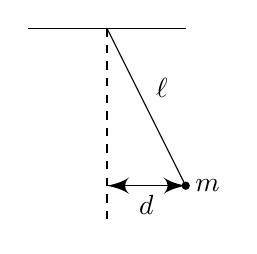
\begin{tikzpicture}
      \draw (-1, 0) -- (1, 0);
      \draw (0, 0) -- (1, -2) node [right] {$m$} node [circ] {} node [pos = 0.5, anchor = south west] {$\ell$};
      \draw [dashed] (0, 0) -- (0, -2.5);
      \draw [->] (0, -2) -- (1, -2) node [below, pos = 0.5] {$d$};
      \draw [->] (1, -2) -- (0, -2);
    \end{tikzpicture}
  \end{center}
  We want to find the period $P$. We know that $P$ could depend on 
  \begin{itemize}
    \item mass $m$: $[m] = M$
    \item length $\ell$: $[\ell] = L$
    \item gravity $g$: $[g] = LT^{-2}$
    \item initial displacement $d$: $[d] = L$
  \end{itemize}
  and of course $[P] = T$.

  We observe that $m, \ell, g$ have independent dimensions, and with the fourth, we can form the dimensionless group $d/\ell$. So the relationship must be of the form
  \[
    P = f\left(\frac{d}{l}\right) m^{p_1}\ell^{p_2}g^{p_3},
  \]
  where $f$ is a dimensionless function. For the dimensions to balance,
  \[
    T = M^{p_1}L^{p_2}L^{p_3}T^{-2p_3}.
  \]
  So $p_1 = 0, p_2 = -p_3 = 1/2$. Then
  \[
    P = f\left(\frac{d}{\ell}\right) \sqrt{\frac{\ell}{g}}.
  \]

  While we cannot find the exact formula, if $\ell$ is quadrupled and $d$ is also quadrupled, the $P$ will double. 
\end{eg}

\section{Forces}
\begin{center}
  \includegraphics[scale=.45]{images/xkcd_experiment.png}\\
  xkcd (Randall Munroe) CC-BY-NC 2.5
\end{center}
\subsection{Force and potential energy in one dimension}
Consider a particle of mass $m$ moving in a straight line with position $x(t)$. Suppose $F = F(x)$, ie. depends on position only. We define the potential energy as follows:
\begin{defi}[Potential energy]
  Given a force field $F = F(x)$, we define the \emph{potential energy} to be a function $V(x)$ such that
  \[
    F = -\frac{\d V}{\d x}.
  \]
  or
  \[
    V = -\int F \;\d x.
  \]
  $V$ includes an arbitrary additive constant.
\end{defi}

The equation of motion is then
\[
  m\ddot{x} = -\frac{\d V}{\d x}.\tag{*}
\]

\begin{prop}
  Suppose the equation of a particle satisfies
  \[
    m\ddot{x} = -\frac{\d V}{\d x}.\tag{*}
  \]
  Then the total energy
  \[
    E = T + V = \frac{1}{2} m\dot{x}^2 + V(x)
  \]
  is conserved, ie. $\dot{E} = 0$.
\end{prop}

\begin{proof}
  \begin{align*}
    \frac{\d E}{\d t} &= m\dot{x}\ddot{x} + \frac{\d V}{\d x}\dot{x}\\
    &= \dot{x}\left(m\ddot{x} + \frac{\d V}{\d x}\right)\\
    &= 0
  \end{align*}
\end{proof}

\begin{eg}
  Consider the harmonic oscillator
  \[
    V = \frac{1}{2} kx^2.
  \]
  Then the equation of motion satisfy
  \[
    m\ddot{x} = -kx.
  \]
  This is the case of, say, Hooke's Law for a spring. But in general, small perturbations near potential wells are also harmonic oscillators.

  The general solution of this is
  \[
    x(t) = A\cos (\omega t) + B\sin (\omega t)
  \]
  with $\omega = \sqrt{k/m}$.

  $A$ and $B$ are arbitrary constants, and are related to the initial position and velocity by $x(0) = A, \dot{x}(0) = \omega B$.
\end{eg}

For a general potential energy $V(x)$, conservation of energy allows us to solve the problem formally:
\[
  E = \frac{1}{2}m\dot{x}^2 + V(x)
\]
Since $E$ is a constant, from this equation, we have
\begin{align*}
  \frac{\d x}{\d t} &= \pm \sqrt{\frac{2}{m}(E - V(x))}\\
  \pm \int \frac{\d x}{\sqrt{\frac{2}{m}(E - V(x))}} &= t - t_0
\end{align*}
To find $x(t)$, we need to do the integral, we need to do the integral and then solve for $x$ - not usually possible by analytical methods, but possible by numerical methods.

\subsection{Motion in a potential}
The graph of the potential energy $V(x)$ gives us a qualitative understanding of the dynamics, eg. is the particle trapped or can it escape to infinity?

\begin{eg}
  Consider $V(x) = m(x^3 - 3x)$. Note that this can be dimensionally consistent even though we add up $x^3$ and $-3x$ if ``3'' has dimensions $L^2$.

  We plot this as follows:
  \begin{center}
    \begin{tikzpicture}
      \draw [->] (-3, 0) -- (3, 0) node [right] {$x$};
      \draw [domain=-2.2:2.2, samples=50] plot (\x, {0.5*(\x*\x*\x - 3*\x)});
      \draw [->] (0, -2) -- (0, 2) node [above] {$M$};
      \node [anchor = north east] {$O$};
      \draw (1, 0) -- (1, -0.1) node [below] {$1$};
      \draw (2, 0) -- (2, -0.1) node [below] {$2$};
      \draw (-1, 0) -- (-1, -0.1) node [below] {$-1$};
      \draw (-2, 0) -- (-2, -0.1) node [below] {$-2$};
    \end{tikzpicture}
  \end{center}

  Suppose we release the particle from rest at $x = x_0$. Then $E = V(x_0)$. We can consider the different cases:
  \begin{itemize}
    \item $x_0 = \pm 1$: Particle stays there for all $t$.
    \item $-1 < x_0 < 2$: Particle oscillates back and forth in potential well
    \item $x_0 < -1$: Particle falls to $x = -\infty$.
    \item $x_0 > 2$: Particle overshoots well and continues to $x = -\infty$.
    \item $x_0 = 2$: Special case: The particle goes towards $x = -1$. How long does it take, and what happens next? Here $E = 2m$, we we noted previously
      \[
        t - t_0 = -\int \frac{\d x'}{\sqrt{\frac{2}{m}(E - V(x'))}}.
      \]
      Let $x = -1 + \varepsilon(t)$. Then
      \begin{align*}
        \frac{2}{m}(E-V(x)) &= 4 - 2(-1 + \varepsilon)^3 + 6(-1 + \varepsilon)\\
        &= 6\varepsilon^2 - 2\varepsilon^3.
      \end{align*}
      So
      \[
        t - t_0 = -\int_3^\varepsilon \frac{\d \varepsilon'}{\sqrt{6\varepsilon'^2 - 2\varepsilon'^3}}
      \]
      Then the integrand is $\propto 1/\varepsilon '$ as $\varepsilon' \to 0$. So it takes infinite time to reach $\varepsilon = 0$, ie. $x = -1$.
  \end{itemize}
\end{eg}
\subsubsection{Equilibrium points}
\begin{defi}[Equilibrium point]
  A particle is in \emph{equilibrium} if it has no tendency to move away. It will stay there for all time. Since $m\ddot{x} = -V'(x)$, the equilibrium points are the stationary points of the potential energy, ie.
  \[
    V'(x_0) = 0;
  \]
\end{defi}

Consider motion near an equilibrium point. Expand $V$ in a Taylor series:
\[
  V(x) \approx V(x_0) + \frac{1}{2}V''(x_0)(x - x_0)^2.
\]
Neglect the higher-order terms. Then the equation of motion is 
\[
  m\ddot{x} = -V''(x_0)(x - x_0).\\
\]

If $V''(x_0) > 0$, then $V$ has a local minimum at $x_0$, and we have the potential of the harmonic oscillator. The equilibrium point is \emph{stable} and the particle oscillates with angular frequency
\[
  \omega = \sqrt{\frac{V''(x_0)}{m}}.
\]
This is only valid for small oscillations. This shows that small oscillations near stable equilibriums are stable.

If $V''(x_0) < 0$, then $V$ has a local maximum at $x_0$. The equilibrium point is unstable. In this case,
\[
  x - x_0 \approx Ae^{\gamma t} + Be^{-\gamma t}
\]
for
\[
  \gamma = \sqrt{\frac{-V''(x_0)}{m}}.
\]
For almost all initial conditions, $A \not= 0$ and the particle will diverge from the equilibrium point, leading to a breakdown of the approximation.

If $V''(x_0) = 0$, then further work is required to determine the outcome.

\begin{eg}
  Consider the simple pendulum.
  \begin{center}
    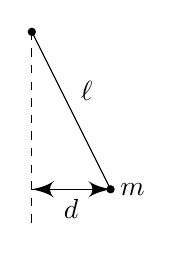
\begin{tikzpicture}
      \draw (0, 0) node [circ] {} -- (1, -2) node [right] {$m$} node [circ] {} node [pos = 0.5, anchor = south west] {$\ell$};
      \draw [dashed] (0, 0) -- (0, -2.5);
      \draw [->] (0, -2) -- (1, -2) node [below, pos = 0.5] {$d$};
      \draw [->] (1, -2) -- (0, -2);
    \end{tikzpicture}
  \end{center}
  Suppose that the pendulum makes an angle $\theta$ with the vertical. The equation of motion is governed by
  \[
    l\ddot{\theta} = -g\sin \theta.
  \]
  The energy is
  \[
    E = T + V = \frac{1}{2}m\ell^2 \dot{\theta}^2 - mg\ell \cos\theta.
  \]
  Therefore $V\propto -\cos\theta$. We have a stable equilibrium at $\theta = 0 $, and unstable equilibrium at $\theta = \pi$.
  \begin{center}
    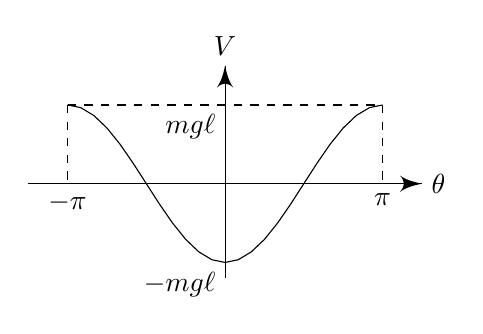
\begin{tikzpicture}
      \draw [domain=-1:1] plot ({2*\x}, {-1 * cos(180 * \x)});
      \draw [->] (-2.5, 0) -- (2.5, 0) node [right] {$\theta$};
      \draw [->] (0, -1.2) -- (0, 1.5) node [above] {$V$};
      \draw [dashed] (-2, 1) -- (-2, 0) node [below] {$-\pi$};
      \draw [dashed] (2, 1) -- (2, 0) node [below] {$\pi$};
      \draw [dashed] (-2, 1) -- (2, 1);
      \node [anchor = north east] at (0, 1) {$mg\ell$};
      \node [anchor = north east] at (0, -1) {$-mg\ell$};
      
    \end{tikzpicture}
  \end{center}
  If $E > mg\ell$, then $\dot{\theta}$ never vanishes and the pendulum makes full circles.
  
  If $E < -mg\ell < E < mg\ell$, then $\dot{\theta}$ vanishes at $\theta = \pm \theta_0$, where $0 < \theta_0 < \pi$< ie. $E = -mg\ell \cos\theta_0$. The pendulum oscillates back and forth. It takes a quarter of a period to reach from $\theta = 0$ to $\theta = \theta_0$. Using the previous general solution, oscillation period $P$ is given by
  \[
    \frac{P}{4} = \int_0^{\theta_0} = \frac{\d \theta}{\sqrt{\frac{2E}{m\ell^2} + \frac{2g}{\ell }\cos\theta}}.
  \]
  Since we know that $E = -mg\ell \cos \theta_0$, we know that
  \[
    \frac{P}{4} = \sqrt{\frac{\ell}{g}}\int_0^{\theta_0} \frac{\d \delta}{\sqrt{2\cos\theta - 2\cos\theta_0}}.
  \]
  The integral is difficult to evaluate in general, but for small $\theta_0$, we can use $\cos\theta \approx 1 - \frac{1}{2}\theta^2$. So
  \[
    P \approx \sqrt{\frac{\ell}{g}}\int_0^{\theta_0}\frac{\d \theta}{\sqrt{\theta_0^2 - \theta^2}} = 2\pi\sqrt{\frac{\ell}{g}}
  \]
  and is independent of the amplitude $\theta_0$. This is of course the result for the harmonic oscillator. 
\end{eg}
\subsubsection{Force and potential energy in three dimensions}
Consider a particle of mass $m$ moving in 3D. The equation of motion is a vector equation
\[
  m\ddot{\mathbf{r}} = \mathbf{F}.
\]
We define the kinetic energy of the particle is
\[
  T = \frac{1}{2}v|\mathbf{v}|^2 = \frac{1}{2}m\dot{\mathbf{r}}\cdot \dot{\mathbf{r}}.
\]
If we want to know how it varies with time, we obtain
\[
  \frac{\d T}{\d t} = m\ddot{\mathbf{r}}\cdot \dot{\mathbf{r}} = \mathbf{F}\cdot \dot{\mathbf{r}} = \mathbf{F}\cdot \mathbf{v}.
\]
This is the power.
\begin{defi}[Power]
  The \emph{power} is the rate at which work is done on a particle by a force. It is given by
  \[
    P = \mathbf{F}\cdot \mathbf{v}.
  \]
\end{defi}
\begin{defi}[Work done]
  The \emph{work done} on a particle by a force is the change in kinetic energy caused by the force. The work done on a particle moving from $\mathbf{r}_1 = \mathbf{r}(t_1)$ to $\mathbf{r}_2 = \mathbf{r}(t_2)$ along a trajectory $C$ is the line integral
  \[
    W = \int_C \mathbf{F}\cdot\d \mathbf{r} = \int_{t_1}^{t_2} \mathbf{F}\cdot \dot{\mathbf{r}}\;\d t = \int_{t_1}^{t_2} P \;\d t.
  \]
\end{defi}

Now we define a particular type of force known as \emph{conservative force} that has many important properties.
\begin{defi}[Conservative force and potential energy]
  A \emph{conservative force} is a force field $\mathbf{F}(\mathbf{r})$ that can be written in the form
  \[
    \mathbf{F} = -\nabla V.
  \]
  $V$ is the \emph{potential energy function}.
\end{defi}

\begin{prop}
  If $\mathbf{F}$ is conservative, then the energy
  \begin{align*}
    E &= T + V\\
    &= \frac{1}{2}m|\mathbf{v}|^2 + V(\mathbf{r})
  \end{align*}
  is conserved. Then the work done is equal to the change in potential energy, and is independent of the path taken between the end points.

  In particular, if we travelled around a closed loop, no work is done.
\end{prop}

\begin{proof}
  \begin{align*}
    \frac{\d E}{\d t} &= m\ddot{\mathbf{r}}\cdot \dot{\mathbf{r}} + \frac{\partial V}{\partial x_i}\frac{\d x_i}{\d t}\\
    &= (m\ddot{\mathbf{r} + \nabla V}\cdot \dot{\mathbf{r}}\\
    &= (m\ddot{\mathbf{r}} - \mathbf{F})\cdot \dot{\mathbf{r}}\\
    &= 0
  \end{align*}
  In this case, the work done is
  \[
    W = \int_C \mathbf{F}\cdot \d \mathbf{r} = -\int_C (\nabla V)\cdot \d \mathbf{r} = V(\mathbf{r}_1) - V(\mathbf{r}_2).
  \]
\end{proof}
\subsection{Central forces}
This is a special class of conservative force, where the potential depends only on the distance from the origin.
\begin{defi}[Central force]
  A central force is a force with a potential $V(r)$ that depends only on the distance from the origin, $r = |\mathbf{r}|$. Note that a central force can be both attractive or repulsive.
\end{defi}

Note the following useful formula
\begin{prop}
  $\nabla r = \hat{\mathbf{r}}$. 
\end{prop}
This is because the direction in which $r$ increases most rapidly is $\mathbf{r}$, and the rate of increase is clearly 1. This can also be proved algebraically:

\begin{proof}
  We know that
  \[
    r^2 = x_1^2 + x_2^2 + x_3^2.
  \]
  Then
  \[
    2r\frac{\partial r}{\partial x_i} = 2x_i.
  \]
  So
  \[
    \frac{\partial r}{\partial x_i} = \frac{x_i}{r} = (\hat{\mathbf{r}})_i.
  \]
\end{proof}

\begin{prop}
  Let $\mathbf{F} = -\nabla V(r)$ be a central force. Then
  \[
    \mathbf{F} = -\nabla V = -\frac{\d V}{\d r} \hat{\mathbf{r}},
  \]
  where $\hat{\mathbf{r}} = \mathbf{r}/r$ is the unit vector in the radial direction pointing away from the origin.
\end{prop}

\begin{proof}
  Continuing the proof above,
  \[
    (\nabla V)_u = \frac{\partial V}{\partial x_i} = \frac{\d V}{\d r} \frac{\partial r}{\partial x_i} = \frac{\d V}{\d r}(\hat{\mathbf{r}})_i
  \]
\end{proof}
Central forces give rise to an additional conserved quantity called \emph{angular momentum}.

\begin{defi}[Angular momentum]
  The \emph{angular momentum} of a particle is
  \[
    \mathbf{L} = \mathbf{r}\times \mathbf{p} = m\mathbf{r}\times \dot{\mathbf{r}}.
  \]
\end{defi}

\begin{prop}
  Angular momentum is conserved by a central force.
\end{prop}

\begin{proof}
  \[
    \frac{\d \mathbf{L}}{\d t} = m\dot{\mathbf{r}} \times \dot{\mathbf{r}} + m\mathbf{r}\times \ddot{\mathbf{r}} = \mathbf{0} + \mathbf{r}\times \mathbf{F} = \mathbf{0}.
  \]
  where the last equality comes from the fact that $\mathbf{F}$ is parallel to $\mathbf{r}$ for a central force.
\end{proof}
In general, for a non-central force, the rate of change of momentum is the \emph{torque}.
\begin{defi}[Torque]
  The \emph{torque} $G$ of a particle is the rate of change of momentum.
  \[
    \mathbf{G} = \frac{\d \mathbf{L}}{\d t} = \mathbf{r}\times \mathbf{F}.
  \]
\end{defi}

Note that $\mathbf{L}$ and $\mathbf{G}$ depends on the choice of origin. For a central force, only the angular momentum about the center of the force is conserved.

\subsection{Gravity}
Gravity is a conservative and central force.
\begin{law}
  If a particle of mass $M$ is fixed at a origin, then a second particle of mass $m$ experiences a potential energy
  \[
    V(r) = -\frac{GMm}{r},
  \]
  where $G \approx \SI{6.67e-11}{\meter\cubed\per\kilogram\per\second\squared}$ is the \emph{gravitational constant}.
  
  The gravitational force experienced is then
  \[
    F = -\nabla V = -\frac{GMm}{r^2}\hat{\mathbf{r}}.
  \]
\end{law}
Since the force is negative, particles are attracted to the origin.

\begin{defi}[Gravitaional potential and field]
  The \emph{gravitational potential} is the gravitational potential energy per unit mass. It is
  \[
    \Phi_g(r) = -\frac{GM}{r}.
  \]
  Note that \emph{potential} is different from \emph{potential energy}.

  The \emph{gravitational field} is the force per unit mass,
  \[
    \mathbf{g} = -\nabla \Phi_g = -\frac{GM}{r^2}\hat{\mathbf{r}}.
  \]
  These are properties of the mass $M$ alone.

  Then the potential energy of a second particle is $V = m\Phi_g$.
\end{defi}

\begin{prop}
  The gravitational potential due to many fixed masses $M_i$ at points $\mathbf{r}_i$ is is
  \[
    \Phi_g(\mathbf{r}) = -\sum_i \frac{GM_i}{|\mathbf{r} - \mathbf{r}_i|}.
  \]
  Again, $V = m\Phi_g$ for a particle of mass $m$.
\end{prop}

\begin{prop}
  The external gravitational potential of a spherically symmetric object of mass $M$ is the same as that of a point particle with the same mass at the center of the object, ie.
  \[
    \Phi_g(r) = -\frac{GM}{r}.
  \]
\end{prop}

\begin{proof}
  cf. Vector Calculus
\end{proof}

\begin{eg}
  If you live on a spherical planet of mass $M$ and radius $R$, and can move only a small distance $z \ll R$ above the surface, then
  \begin{align*}
    V(r) &= V(R + z)\\
    &= -\frac{GMm}{r + z}\\
    &= -\frac{GMm}{r}\left(1 - \frac{z}{R} + \cdots\right)\\
    &\approx \text{const.} + \frac{GMm}{R^2}z\\
    &= \text{const.} + mgz.
  \end{align*}
  where $g = GM/R^2 \approx \SI{9.8}{\meter\per\second\squared}$ for Earth.
\end{eg}

\begin{eg}
 How fast do we need to jump to escape the gravitational pull of the Earth? If we jump upwards with speed $v$ from the surface, then
 \[
   E = T + V = \frac{1}{2}mv^2 - \frac{GMm}{R}.
 \]
 Since after escape, we have $T \geq 0$ and $V = 0$, and energy is conserved, we must have $E \geq 0$ from the very beginning. ie.
 \[
   v > v_{esc} = \sqrt{\frac{2GM}{R}}.
 \]
\end{eg}
\subsubsection{Inertial and gravitational mass}
Mass appears in two equations:
\[
  m_i\ddot{\mathbf{r}} = \mathbf{F}\quad \text{ (inertial mass)}
\]
and
\[
  \mathbf{F} = -\frac{GM_gm_g}{r^2}\hat{\mathbf{r}}\quad\text{ (gravitational mass)}.
\]
and they play totally different roles. Conceptually, these are quite different, but experiment shows that they are indeed equivalent to each other, ie. $m_i = m_g$, with an accuracy of $10^{-12}$ or better.

This is only explained by Einstein's general theory of relativity.

We can further distinct the gravitational mass by ``passive'' and ``active'', ie. the amount of gravitational field generated by a particle ($M$), and the amount of gravitational force received by a particle ($m$), but they are still equal, and we end up calling all of them ``mass''.

\subsection{Electromagnetism}
\begin{notation}[Electric and magnetic field]\leavevmode
   \begin{enumerate}
    \item $\mathbf{E}(\mathbf{r}, t)$ is the electric field;
    \item $\mathbf{B}(\mathbf{r}, t)$ is the magnetic field;
    \item $\mathbf{v} = \dot{\mathbf{r}}$ is the velocity of the particle.
  \end{enumerate}
\end{notation}
\begin{law}[Lorentz force law]
  The \emph{electromagnetic force} experienced by a particle with electric charge $q$ is
  \[
    \mathbf{F} = q(\mathbf{E} + \mathbf{v}\times \mathbf{B}).
  \]
\end{law}

\begin{law}
  The electron has charge
  \[
    q_e = \SI{-1.6e-19}{\coulomb}
  \]
  and other particles' charges are integer multiples of this unit (unless you are a quark).
\end{law}

\begin{law}
  For time-independent fields, $\mathbf{E}$ can be written as
  \[
    \mathbf{E} = -\nabla \Phi_e,
  \]
  where $\Phi_e(\mathbf{r})$ is the \emph{electrostatic potential}.
  The electric force $q\mathbf{E}$ is then conserved.
\end{law}
\begin{defi}[Electrostatic potential]
  The electrostatic potential is a function $\Phi_e(\mathbf{r})$ such that
  \[
    \mathbf{E} = -\nabla \Phi_e.
  \]
\end{defi}

Note that $\mathbf{E}$ is conservative, and $B$ acts perpendicular to the velocity, and so does no work. So
\begin{prop}
  For time independent $\mathbf{E}(\mathbf{r})$ and $\mathbf{B}(\mathbf{r})$, the energy
  \[
    E = T + V = \frac{1}{2}m|\mathbf{v}|^2 + q\Phi_e
  \]
  is conserved.
\end{prop}

\begin{proof}
  \begin{align*}
    \frac{\d E}{\d t} &= m\ddot{\mathbf{r}}\cdot \dot{\mathbf{r}} + q(\nabla \Phi_e)\cdot \dot{\mathbf{r}}\\
    &= (m\ddot{\mathbf{r}} - q\mathbf{E}) \cdot \dot{\mathbf{r}}\\
    &= (q\dot{\mathbf{r}}\times \mathbf{B})\cdot \dot{\mathbf{r}}\\
    &= 0
  \end{align*}
\end{proof}

\subsubsection{Point charges}
\begin{law}[Columb's law]
  A particle of charge $Q$, fixed at the origin, produces an electrostatic potential
  \[
    \Phi_e = \frac{Q}{4\pi\varepsilon_0 r},
  \]
  where $\varepsilon_0 \approx \SI{8.85e-12}{\per\meter\cubed\per\kilogram\second\squared\coulomb\squared}$.

  The corresponding electric field is 
  \[
    \mathbf{E} = -\nabla \Phi_e = \frac{Q}{4\pi\varepsilon_0} \frac{\hat{\mathbf{r}}}{r^2}.
  \]
  The resulting force on a particle of charge $q$ is
  \[
    \mathbf{F} = q\mathbf{E} = \frac{Qq}{4\pi\varepsilon_0}\frac{\hat{\mathbf{r}}}{r^2}.
  \]
\end{law}
\begin{defi}[Electric constant]
  $\varepsilon_0$ is the \emph{electric constant} or \emph{vacuum permittivity} or \emph{permittivity of free space}.
\end{defi}

Electrostatic forces are closely analogous to gravitational forces, but there is an important difference: charges can be positive or negative. Thus electrostatic forces can be either attractive or repulsive, whereas gravity is always attractive.

\subsubsection{Motion in a uniform magnetic field}
Set $\mathbf{E} = \mathbf{0}$ and choose axes such that $\mathbf{B} = (0, 0, B)$ is constant.

According to the Lorentz force law, $\mathbf{F} = q(\mathbf{E} + \mathbf{v}\times \mathbf{B})$. The components of the equation of motion are
\begin{align*}
  m\ddot{x} &= qB\dot{y}\tag{1}\\
  m\ddot{y} &= -qB\dot{x}\tag{2}\\
  m\ddot{z} &= 0
\end{align*}
So we have a uniform motion parallel to $\mathbf{B}$.

There are many ways to solve this system of equations. Here we solve it using complex numbers.

Let $\zeta = x + iy$. Then (1) + (2)$i$ gives
\[
  m\ddot{\zeta} = -iqB\dot{\zeta}.
\]
Then the solution is
\[
  \zeta = \alpha e^{-\omega t} + \beta,
\]
where $\omega = qB/m$ is the \emph{gyrofrequency}, and $\alpha$ and $\beta$ are complex integration constants. We see that the particle goes in circles, with center $\beta$ and radius $\alpha$.

We can choose coordinates such that, at $t = 0$, $\mathbf{r} = 0$ and $\dot{\mathbf{r}} = (0, v, w)$, ie.~$\zeta = 0$ and $\dot{\zeta} = iv$, and $z = 0$ and $\cdot z = w$.

The solution is then
\[
  \zeta = R(1 - e^{-i\omega t}).
\]
with $R = v/\omega = (mv)/(qB)$ is the \emph{gyroradius} or \emph{Larmor radius}. Alternatively,
\begin{align*}
  x &= R(1 - \cos \omega t)\\
  y &= R\sin \omega t\\
  z &= wt.
\end{align*}
This is circular motion in the plane perpendicular to $\mathbf{B}$:
\[
  (x - R)^2 + y^2 = R^2,
\]
combined with uniform motion parallel to $\mathbf{B}$, ie.~a helix.

We can also have a vectorial treatment: Start with
\[
  m\ddot{\mathbf{e}} = q\dot{\mathbf{r}}\times \mathbf{B}
\]
Let $\mathbf{B} = B\mathbf{n}$ with $|\mathbf{n}| = 1$. Then
\[
  \ddot{\mathbf{r}} = \omega \dot{\mathbf{r}}\times \mathbf{n},
\]
with our gyrofrequency $\omega = qB/m$. We integrate once, assuming $\mathbf{r}(0) = \mathbf{0}$ and $\dot{\mathbf{r}}(0) = \mathbf{v}_0$.
\[
  \dot{\mathbf{r}} = \omega \mathbf{r} \times \mathbf{n} + \mathbf{v}_0. \tag{$*$}
\]
Project $(*)$ parallel to and perpendicular to $\mathbf{B}$:

First dot $(*)$ with $\mathbf{n}$:
\[
  \dot{\mathbf{r}}\cdot \mathbf{n} = \mathbf{v}_0\cdot \mathbf{n} = w = \text{const}.
\]
We integrate again to obtain
\[
  \mathbf{r}\cdot \mathbf{n} = wt.
\]
Then write $\mathbf{r} = (\mathbf{r}\cdot \mathbf{n})\mathbf{n} + \mathbf{r}_\bot$, with $\mathbf{r}_\bot \cdot \mathbf{n} = 0$.

The perpendicular component of $(*)$ gives
\[
  \dot{\mathbf{r}}_\bot = w\mathbf{r}_\bot \times \mathbf{n} + \mathbf{v}_0 - (\mathbf{v}_0\cdot \mathbf{n})\mathbf{n}).
\]
We solve this by differentiating again to obtain
\[
  \ddot{\mathbf{r}}_\bot = \omega \dot{\mathbf{r}}_\bot \times \mathbf{n} = -\omega^2 \mathbf{r}_\bot + \omega \mathbf{v}_0 \times \mathbf{n},
\]
which we can solve using particular integrals and complementary functions.

\subsection{Friction}
Energy is conserved at an atomic level, but does not appear to be conserved in many everyday processes. This is described by \emph{friction}. We divide them into different categories:
\begin{defi}[Dry friction]
  When solid objects are in contact, a \emph{normal reaction force} $\mathbf{n}$ (perpendicular to the contact surface) prevents them from interpenetrating, while a \emph{frictional force} $\mathbf{F}$ (tangential to the surface) resists relative tangential motion (sliding or slipping).
  \begin{center}
    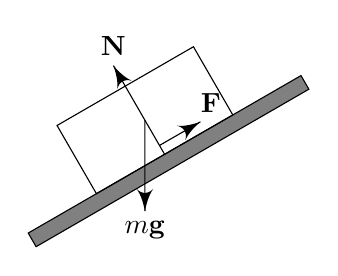
\begin{tikzpicture}[rotate = 30]
      \draw [fill=gray] (-2, 0) rectangle (2, -0.2);
      \draw (-1, 1) rectangle (1, 0);
      \draw [->] (0, 0) -- (0, 1.3) node [above] {$\mathbf{N}$};
      \draw [->] (0, 0.13) -- (0.6, 0.13) node [anchor = south west] {$\!\!\mathbf{F}$};
      \draw [->] (0, 0.5) -- (-0.577, -0.5) node [below] {$m\mathbf{g}$};
    \end{tikzpicture}
  \end{center}
  If no sliding occurs, then we have \emph{static friction} of
  \[
    |\mathbf{F}| \leq \mu_s |\mathbf{N}|,
  \]
  where $\mu_s$ is the \emph{coefficient of static friction}.

  If sliding occurs, then we have \emph{kinetic friction} of 
  \[
    |F| = \mu_k |\mathbf{N}|,
  \]
  where $\mu_k$ is the \emph{coefficient of kinetic friction}.

  These coefficients are measures of roughness and depend on the two surfaces involved. For example, Teflon on Teflon has coefficient of around 0.04, what rubber on asphalt has about 0.8.

  Usually, $\mu_s > \mu_k > 0$.

  A hypothetical perfectly smooth surface has $\mu_s = \mu_k =0$.
\end{defi}

\begin{defi}[Fluid drag]
  When a solid object moves through a fluid (ie. liquid or gas), it experiences a \emph{drag force}.

  There are two important regimes.

  \begin{enumerate}
    \item Linear drag: for small things in viscous fluids moving slowly, eg. a single cell organism in water,
      \[
        \mathbf{F} = -k_1 \mathbf{v}.
      \]
      where $\mathbf{v}$ is the velocity of the object relative to the fluid, and $k_1> 0$ is a constant. For a sphere of radius $R$, Stoke's Law gives
      \[
        k_1 = 6\pi \mu R,
      \]
      where $\mu$ is the viscosity of the fluid.
    \item Quadratic drag: for large objects moving rapidly in less viscous fluid, eg. cars or tennis balls in air,
      \[
        \mathbf{F} = -k_2|\mathbf{v}|\mathbf{v}.
      \]
      Note that we have $|\mathbf{v}|\mathbf{v}$ because we want the square of the speed and the direction of the velocity. It can be (probably) more clearly written as $|\mathbf{v}|^2 \hat{\mathbf{v}}$.

  \end{enumerate}
  In either case, the object loses energy. The power exerted be the drag force is
  \[
    \mathbf{F}\cdot \mathbf{v} = \begin{cases} -k_1|\mathbf{v}|^2\\-k_2 |\mathbf{v}|^3 \end{cases}
  \]
\end{defi}
\begin{eg}
  Consider a projectile moving in a uniform gravitational field and experiencing a linear drag force.

  At $t = 0$, we through the projectile with velocity $\mathbf{u}$ from $\mathbf{x} = \mathbf{0}$.

  The equation of motion is
  \[
    m\frac{\d \mathbf{v}}{\d t} = m\mathbf{g} - k\mathbf{v}.
  \]
  We first solve for $\mathbf{v}$, and then deduce $\mathbf{x}$.

  We use an integrating factor $\exp(\frac{k}{m}t)$ to obtain
  \begin{align*}
    \frac{\d }{\d t} \left(e^{kt/m}\mathbf{v}\right) &= e^{kt/m} \mathbf{g}\\
    e^{kt/m} \mathbf{v}&= \frac{m}{k}e^{kt/m}\mathbf{g} + \mathbf{c}\\
    \mathbf{v} &= \frac{m}{k}\mathbf{g} + \mathbf{c} e^{-kt/m}
  \end{align*}
  Since $\mathbf{v} = \mathbf{u}$ at $t = 0$, $\mathbf{c} = \mathbf{u} - \frac{m}{k}\mathbf{g}$. So
  \[
    \mathbf{v} = \dot{\mathbf{x}} = \frac{m}{k}\mathbf{g} + \left(\mathbf{u} - \frac{m}{k}\mathbf{g}\right)e^{-kt/m}.
  \]
  Integrating once gives
  \[
    \mathbf{x} = \frac{m}{k}\mathbf{g}t - \frac{m}{k}\left(\mathbf{u} - \frac{m}{k} g\right) e^{-kt/m} + \mathbf{d}.
  \]
  Since $\mathbf{x} = \mathbf{0}$ at $t = 0$. So
  \[
    \mathbf{d} = \frac{m}{k}\left(\mathbf{u} - \frac{m}{k}\mathbf{g}\right).
  \]
  So
  \[
    \mathbf{x} = \frac{m}{k}\mathbf{g}t + \frac{m}{k}\left (\mathbf{u} - \frac{m}{k}\mathbf{g}\right)(1 - e^{-kt/m}).
  \]
  In component form, let $\mathbf{x} = (x, y)$, $\mathbf{u} = (u\cos \theta, u\sin \theta)$, $\mathbf{g} = (0, -g)$. So
  \begin{align*}
    x &= \frac{mu}{k}\cos \theta (1 - e^{-kt/m})\\
    z &= -\frac{mgt}{k} + \frac{m}{k}\left(u\sin \theta + \frac{mg}{k}\right)(1 - e^{-kt/m}).
  \end{align*}
  We can characterize the strength of the drag force by the dimensionless constant $ku/(mg)$, with a larger constant corresponding to a larger drag force. 
\end{eg}
\subsubsection{Effect of damping on small oscillations}
Friction or drag causes oscillations about a potential minimum to be damped out. Energy is continually lost until the system comes to rest at the stable equilibrium.

\begin{eg}
  If a linear drag force is added to a harmonic oscillator, then the equation of motion becomes
  \[
    m\ddot{\mathbf{x}} = -m\omega^2 \mathbf{x} - k\dot{\mathbf{x}},
  \]
  where $\omega$ is the angular frequency of the oscillator in the absence of damping. Rewrite as
  \[
    \ddot{\mathbf{x}} + 2\gamma \dot{\mathbf{x}} + \omega^2 x = 0,
  \]
  where $\gamma = k/2m > 0$. Solutions are $x = e^{\lambda t}$, where
  \[
    \lambda^2 + 2\gamma \lambda + \omega^2,
  \]
  or
  \[
    \lambda = -\gamma \pm \sqrt{\gamma^2 - \omega^2}.
  \]
  If $\gamma > \omega$ (overdamped oscillator), roots are real and negative. So we have exponential decay.

  If $0 < \gamma < \omega$ (underdamped oscillator), roots are complex with $\re(\lambda) = -\gamma$. So we have decaying oscillations.

  For details, refer to Differential Equations.
\end{eg}

\section{Orbits}
\begin{center}
  \includegraphics[scale=.75]{images/xkcd_orbital_mechanics.png}\\
  xkcd (Randall Munroe) CC-BY-NC 2.5
\end{center}
We will study the motion in 3D of a particle in a central force,
\[
  m\ddot{\mathbf{r}} = -\nabla V(r).
\]
The angular momentum $\mathbf{L} = m\mathbf{r}\times \dot{\mathbf{r}}$ is a constant vector, as previously shown. Furthermore $\mathbf{L}\cdot \mathbf{r} = 0$. Therefore, the motion takes place in a plane passing through the origin, and perpendicular to $\mathbf{L}$.

\subsection{Polar coordinates in the plane}
We choose our axes such that the orbital plane is $z = 0$. We introduce polar coordinates $(r, \theta)$:
\[
  x = r\cos\theta, \quad y = r\sin \theta.
\]
\begin{notation}
  We define unit vectors in the directions of increasing $r$ and increasing $\theta$:
  \[
    \hat{\mathbf{r}} = \begin{pmatrix}\cos \theta\\ \sin \theta\end{pmatrix}, \quad \hat{\boldsymbol\theta} = \begin{pmatrix}-\sin \theta\\\cos\theta \end{pmatrix}.
  \]
  \begin{center}
    \begin{tikzpicture}
      \draw [->] (0, 0) -- (4, 0) node [right] {$x$};
      \draw [->] (0, 0) -- (0, 3) node [above] {$y$};
      \draw (0, 0) -- (2, 1.5) node [circ]{} node [pos = 0.5, anchor = south east] {$r$};
      \draw [->] (2, 1.5) -- (2.5, 1.875) node [anchor = south west] {$\hat{\mathbf{r}}$};
      \draw [->] (2, 1.5) -- (1.625, 2) node [anchor = south east] {$\hat{\boldsymbol\theta}$};
      \draw (0.7, 0) arc (0:36.87:0.7);
      \node at (0.9, 0.3) {$\theta$};
    \end{tikzpicture}
  \end{center}
  They form an orthonormal basis at each point, but depends on position:
\end{notation}
\begin{prop}
  \begin{align*}
    \frac{\d \hat{\mathbf{r}}}{\d \theta} &= \begin{pmatrix} -\sin \theta\\ \cos \theta\end{pmatrix} = \hat{\boldsymbol\theta}\\
    \frac{\d \hat{\boldsymbol\theta}}{\d \theta} &= \begin{pmatrix}-\cos \theta\\ -\sin \theta\end{pmatrix} = -\hat{\mathbf{r}}.
  \end{align*}
\end{prop}

\begin{prop}
  For each particle with trajectory $\mathbf{r}(t)$, the polar coordinates $r$ and $\theta$ depend on $t$, and so do the polar unit vectors. By the chain rule,
  \[
    \frac{\d \hat{\mathbf{r}}}{\d t} = \dot{\theta}\hat{\boldsymbol\theta},\quad \frac{\d \hat{\boldsymbol\theta}}{\d t} = -\dot{\theta} \hat{\mathbf{r}}.
  \]
  In terms of the polar unit vectors, 
  \[
    \mathbf{r} = r\hat{\mathbf{r}}.
  \]
  The velocity is
  \[
    \dot{\mathbf{r}} = \dot{r} \hat{\mathbf{r}} + r\dot{\theta} \hat{\boldsymbol\theta}.
  \]
  The acceleration is
  \begin{align*}
    \ddot{\mathbf{r}} &= \ddot{r} \hat{\mathbf{r}} + \dot{r}\dot{\theta}\hat{\boldsymbol\theta} + \dot{r}\dot{\theta}\hat{\boldsymbol\theta} + r\ddot{\theta}\hat{\boldsymbol\theta} - r\dot{\theta}^2\hat{\mathbf{r}}\\
    &= (\ddot{r} - r\dot{\theta}^2)\hat{\mathbf{r}} + (r\ddot{\theta} + 2\dot{r}\dot{\theta})\hat{\boldsymbol\theta}.
  \end{align*}
\end{prop}

\begin{defi}[Radial and angular velocity]
  $\dot{r}$ is the \emph{radial velocity}, and $\dot{\theta}$ is the \emph{angular velocity}.
\end{defi}

\begin{eg}[Uniform motion in a circle]
  $\dot{r} = 0$, $\dot{\theta} = \omega = $ const.  So $\dot{\mathbf{r}} = r\omega\hat{\boldsymbol\theta}$.

  The speed is 
  \[
    v = |\dot{\mathbf{r}}| = r|w| = \text{ const}.
  \]
  The acceleration is
  \[
    \ddot{\mathbf{r}} = -r\omega^2 \hat{\mathbf{r}}.
  \]
  In order to make a particle of mass $m$ move uniformly in a circle, we must supply a ``centripetal force'' $mv^2/r$ towards the center.
\end{eg}

\subsection{Motion in a central force field}
Since $V = V(r)$, $\mathbf{F} = -\nabla V = \frac{\d V}{\d r} \hat{\mathbf{r}}$.

So Newton's 2nd law in polar coordinates is
\[
  m(\ddot{r} - r\dot{\theta}^2)\hat{\mathbf{r}} + m(r\ddot{\theta} + 2\dot{r}\dot{\theta})\hat{\boldsymbol\theta} = -\frac{\d V}{\d r}\hat{\mathbf{r}}.
\]
The $\theta$ component of this equation is
\[
  m(r\ddot{\theta} - 2\dot{r}\dot{\theta}) = 0.
\]
So
\[
  \frac{1}{r}\frac{\d }{\d t}(mr^2 \dot{\theta}) = 0.
\]
Write $L = mr^2 \dot{\theta}$. This is the $z$ component (ie. the only component) of the conserved angular momentum $\mathbf{L}$:
\begin{align*}
  \mathbf{L} &= m\mathbf{r}\times \dot{\mathbf{r}}\\
  &= mr\hat{\mathbf{r}}\times (\dot{r}\hat{\mathbf{r}} + r\dot{\theta}\hat{\boldsymbol\theta})\\
  &= mr^2 \dot{\theta}\; \hat{\mathbf{r}}\times \hat{\boldsymbol\theta}\\
  &= mr^2 \dot{\theta}\; \hat{\mathbf{z}}.
\end{align*}
So are above equation states that $L$ is constant, which is consistent with the conservation of angular momentum.

Introduce the angular momentum per unit mass:
\begin{notation}[Angular momentum per unit mass]
  The \emph{angular momentum per unit mass} is
  \[
    h = \frac{L}{m} = r^2\dot\theta = \text{const.}
  \]
\end{notation}
The radial ($r$) component of the equation of motion is
\[
  m(\ddot{r} - r\dot{\theta}^2) = -\frac{\d V}{\d r}.
\]
We eliminate $\dot{\theta}$ using $r^2\dot{\theta} = h$ to obtain
\[
  m\ddot{r} = -\frac{\d V}{\d r} + \frac{mh^2}{r^3} = -\frac{\d V_{\text{eff}}}{\d r},
\]
where 
\[
  V_{\text{eff}}(r) = V(r) + \frac{mh^2}{2r^2}.
\]
We have reduced the problem to 1D motion in an (effective) potential - as studied previously.

The total energy of the particle is
\begin{align*}
  E &= \frac{1}{2}m|\dot{\mathbf{r}}|^2 + V(r)\\
  &= \frac{1}{2}m(\dot{r}^2 + r^2\dot{\theta}^2) + V(r)\\
  \intertext{(since $\dot{\mathbf{r}} = \dot{r}\hat{\mathbf{r}} + r\dot{\theta}\hat{\boldsymbol\theta}$, and $\hat{\mathbf{r}}$ and $\hat{\boldsymbol\theta}$ are orthogonal)}
  &= \frac{1}{2}m\dot{r}^2 + \frac{mh^2}{2r^2} + V(r)\\
  &= \frac{1}{2}m\dot{r}^2 + V_{\text{eff}}(r).
\end{align*}

\begin{eg}
  Consider an attractive force following the inverse-square law (eg. gravity). Here
  \[
    V = -\frac{mk}{r},
  \]
  for some constant $k$. So
  \[
    V_{\text{eff}} = -\frac{mk}{r} + \frac{mh^2}{2r^2}.
  \]
  We have two terms of opposite signs and different dependencies on $r$. For small $r$, the second term dominates and $V_{\text{eff}}$ is large. For large $r$, the first term dominates. Then $V_{\text{eff}}$ asymptotically approaches $0$ from below.

  \begin{center}
    \begin{tikzpicture}[xscale=0.5]
      \draw (0, 0) -- (8, 0) node [right] {$r$};
      \draw (0, -2) -- (0, 2) node [above] {$V_{\text{eff}}$};
      \draw [samples=70, domain=0.5:7.8] plot (\x, {-3/\x + 2/(\x*\x)});

      \draw [dashed] (1.33, -1.125) -- (0, -1.125) node [left] {$E_{\min}$};
      \draw [dashed] (1.33, -1.125) -- (1.33, 0) node [above] {$r_*$};
    \end{tikzpicture}
  \end{center}

  The minimum of $V_{\text{eff}}$ is at
  \[
    r_{*} = \frac{h^2}{k},\quad E_{\text{min}} = -\frac{mk^2}{2h^2}.
  \]
  We have a few possible types of motion:
  \begin{itemize}
    \item If $E = E_{\min}$, then $r$ remains at $r_*$ and $\dot{\theta} h/r^2$ is constant. So we have a uniform motion in a circle.
    \item If $E_{\min} < E < 0$, then $r$ oscillates and $\dot{r}=h/r^2$ does also. This is a non-circular, bounded orbit.

      \begin{defi}[Periapsis, apoapsis and apsides]
        The points of minimum and maximum $r$ in such an orbit are called the \emph{periapsis} and \emph{apoapsis}. They are collectively known as the \emph{apsides}.
      \end{defi}

      \begin{defi}[Perihelion and aphelion]
        For an orbit around the Sun, the periapsis and apoapsis are known as the \emph{perihelion} and \emph{aphelion}.
      \end{defi}
  
      In particular
      \begin{defi}[Perigee and apogee]
        The perihelion and aphelion of the Earth are known as the \emph{perigee} and \emph{apogee}.
      \end{defi}

    \item If $E \geq 0$, then $r$ comes in from $\infty$, reaches a minimum, and returns to infinity. This is an unbound orbit.
  \end{itemize}

  In the case of motion in an inverse square force, the trajectories are conic sections (circles, ellipses, parabolae and hyperbolae).
\end{eg}

\subsubsection{Stability of circular orbits}
Here we can deduce the stability of circular orbits. It is particularly important that the orbit in an inverse square force is stable!

Now consider a general potential energy $V(r)$. We have to answer two questions:
\begin{itemize}
  \item Do circular orbits exist?
  \item If they do, are they stable?
\end{itemize}

For a circular orbit, $r = r_* =$ const for some value of $h\not= 0$ (if $h\not = 0$, then the object is just standing still!).

Since $\ddot{r} = 0$ constant $r$, we require
\[
  V'_{\text{eff}}(r_*) = 0.
\]

The orbit is stable if $r_*$ is a minimum of $V_{\text{eff}}$, ie.
\[
  V_{\text{eff}}''(r_*) > 0.
\]
In terms of $V(r)$, we require
\[
  V'(r_*) = \frac{mh^2}{r_*^3}
\]
and is stable for
\[
  V''(r_*) + \frac{3mh^2}{r_*^4} = V''(r_*) + \frac{3}{r_*}V'(r_*) > 0.
\]
In terms of the radial force $F(r) = -V'(r)$, the orbit is stable if
\[
  F''(r_*) + \frac{3}{r}F(r_*) < 0.
\]
\begin{eg}
  Consider a central force with
  \[
    V(r) = -\frac{mk}{r^p}
  \]
  for some $k, p > 0$. Then
  \[
    V''(r) + \frac{3}{r}V'(r) = \big( -p(p + 1) + 3p\big)\frac{mk}{r^{p + 2}} = p(2-p)\frac{mk}{r^{p + 2}}.
  \]
  So circular orbits are stable for $p < 2$. This is illustrated by the graphs of $V_{\text{eff}}(r)$ for $p = 1$ and $p = 3$. 
  \begin{center}
    \begin{tikzpicture}[xscale=0.5]
      \draw (0, 0) -- (8, 0);
      \draw (0, -2) -- (0, 2) node [above] {$V_{\text{eff}}$};
      \draw [blue, samples=10, domain=0.5:1.5] plot (\x, {-3/\x + 2/(\x*\x)});
      \draw [blue, domain=1.5:7.8] plot (\x, {-3/\x + 2/(\x*\x)}) node [right] {$p = 1$};


      \draw [red, dashed, samples=70, domain=0.4:7.8] plot (\x, {-0.6/(\x*\x*\x) + 1.2/(\x*\x)}) node [right] {$p = 3$};
    \end{tikzpicture}
  \end{center}
\end{eg}

\subsection{Equation of the shape of the orbit}
In general, we could determine $r(t)$ by integrating the energy equation
\begin{align*}
  E &= \frac{1}{2}m\dot{r}^2 + V_{\text{eff}}(r)\\
  t &= \pm \sqrt{\frac{m}{2}}\int \frac{\d r}{\sqrt{E - V_{\text{eff}(r)}}}
\end{align*}
However, this is usually not practical, because we can't do the integral.

It is usually much easier to find the shape $r(\theta)$ of the orbit.

We can usually simply the equation by introducing the new variable
\begin{notation}
  \[
    u = \frac{1}{r}.
  \]
\end{notation}
Then
\[
  \dot{r} = \frac{\d r}{\d \theta}\dot{\theta} = \frac{\d r}{\d \theta}\frac{h}{r^2} = -h\frac{\d u}{\d \theta}.
\]
Then
\[
  \ddot{r} = \frac{\d }{\d t}\left(-h \frac{\d u}{\d \theta}\right) = -h\frac{\d ^2 u}{\d \theta^2}\dot{\theta} = -h\frac{\d ^2u}{\d \theta^2}\frac{h}{r^2} = -h^2u^2\frac{\d^2 u}{\d \theta^2}.
\]
This doesn't look very linear with $u^2$, but it will help linearizing the equation when we put in other factors.

The radial equation of motion 
\[
  m\ddot{r} - \frac{mh^2}{r^3} = F(r)
\]
then becomes
\begin{prop}[Binet's equation]
  \[
    -mh^2u^2\left(\frac{\d^2u}{\d \theta^2}+ u\right) = F\left(\frac{1}{u}\right).
  \]
\end{prop}
For an inverse square force, $F(1/u)$ is proportional to $u^2$, and the equation is linear!

Given $F(r)$, we aim to solve this second order ODE for $u(\theta)$. If needed, we can then work out the time-dependence via
\[
  \dot{\theta} = hu^2.
\]
\subsection{The Kepler problem}
\subsubsection{Shapes of orbits}
For a planet orbiting the sun,
\[
  V(r) = \frac{mk}{r},\quad F(r) = -\frac{mk}{r^2}
\]
with $k = GM$.
(For the Coulomb attraction of opposite charges, we have the same equation with $\displaystyle k = -\frac{Qq}{4\pi\epsilon_0 m}$.)

Binet's equation then becomes linear, and
\[
  \frac{\d^2 u}{\d \theta^2} + u = \frac{k}{h^2}.
\]
We write the general solution as
\[
  u = \frac{k}{h^2} + A\cos(\theta - \theta_0),
\]
where $A \geq 0$ and $\theta_0$ are arbitrary constants.

If $A = 0$, then $u$ is constant, and the orbit is circular. Otherwise, $u$ reaches a maximum at $\theta = \theta_0$. This is the periapsis. We now re-define polar coordinates such that the periapsis is at $\theta = 0$. Then
\begin{prop}
  The orbit of a planet around the sun is given by
  \[
    r = \frac{\ell}{1 + e\cos \theta},\tag{$*$}
  \]
  with $\ell = h^2/k$ and $e = Ah^2/k$. This is the polar equation of a conic, with a focus (the sun) at the origin.
\end{prop}

\begin{defi}[Eccentricity]
  The dimensionless parameter $e \geq 0$ in the equation of orbit is the \emph{eccentricity} and determines the shape of the orbit.
\end{defi}

($*$) can be re-written in Cartesian coordinates with $x = r\cos \theta$ and $y = r\sin \theta$ to obtain
\[
  (1 - e^2)x^2 + 2e\ell x + y^2 = \ell^2.\tag{$\dagger$}
\]
There are two different possibilities:
\begin{itemize}
  \item Ellipse: ($0\leq e < 1$). $r$ is bounded by
    \[
      \frac{\ell}{1 + e} \leq r \leq \frac{\ell}{1 - e}.
    \]
    ($\dagger$) can be put into the equation of an ellipse centered on $(-ea, 0)$,
    \[
      \frac{(x + ea)^2}{a^2} + \frac{y^2}{b^2} = 1,
    \]
    where $\displaystyle a = \frac{\ell}{1 - e^2}$ and $\displaystyle b = \frac{\ell}{\sqrt{1 - e^2}}\leq a$.
    \begin{center}
      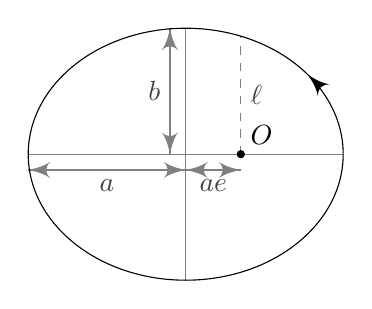
\begin{tikzpicture}
        \draw [gray] (-2, 0) -- (2, 0);
        \draw [gray] (0, -1.6) -- (0, 1.6);
        \draw [gray, ->] (0.7, -0.2) -- (0, -0.2) node [gray!50!black, pos = 0.5, below] {$ae$};
        \draw [gray, ->] (0, -0.2) -- (0.7, -0.2);
        \draw [gray, ->] (-0.2, 0) -- (-0.2, 1.6) node [gray!50!black, pos = 0.5, left] {$b$};
        \draw [gray, ->] (-0.2, 1.6) -- (-0.2, 0);

        \draw [gray, ->] (0, -0.2) -- (-2, -0.2) node [gray!50!black, pos = 0.5, below] {$a$};
        \draw [gray, ->] (-2, -0.2) -- (0, -0.2);
        \draw [gray, dashed] (0.7, 0) -- (0.7, 1.5) node [gray!50!black, pos = 0.5, right] {$\ell$};

        \draw (.7, 0) node [anchor = south west] {$O$} node [circ] {};
        \draw [->-=0.1] (0, 0) circle [x radius = 2, y radius = 1.6];
      \end{tikzpicture}
    \end{center}

    $a$ and $b$ are the semi-major and semi-minor axis. $\ell$ is the semi-latus rectum 
    One focus of the ellipse is at the origin. If $e = 0$, then $a = b = \ell$ and the ellipse is a circle.

  \item Hyperbola: ($e > 1$). For $e > 1$, $r\to \infty$ as $\theta \to \pm \alpha$, where $\alpha = \cos^{-1}(1/e)\in (\pi/2, \pi)$. Then ($\dagger$) can be put into the equation of a hyperbola centered on $(ea, 0)$,
    \[
      \frac{(x - ea)^2}{a^2} - \frac{y^2}{b^2} = 1,
    \]\
    with $\displaystyle a = \frac{\ell}{e^2 - 1}$, $\displaystyle b = \frac{\ell}{\sqrt{e^2 - 1}}$.

    \begin{center}
      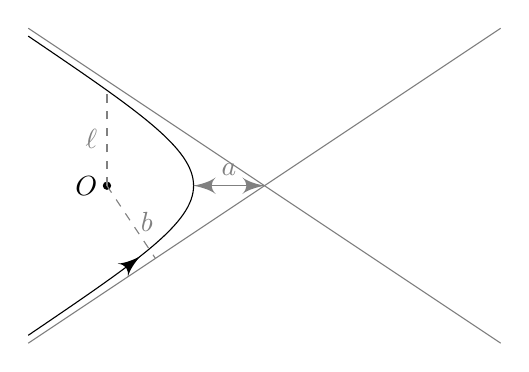
\begin{tikzpicture}
        \draw [gray] (-3, -2) -- (3, 2);
        \draw [gray] (3, -2) -- (-3, 2);
        \draw [->-=0.3] (-3, -1.9) .. controls (-0.2, 0) .. (-3, 1.9);
        \draw [gray, ->] (0, 0) -- (-0.9, 0);
        \draw [gray, ->] (-0.9, 0) -- (0, 0) node [pos = 0.5, above] {$a$};
        \node at (-2, 0) [circ] {};
        \node at (-2, 0) [left] {$O$};
        \draw [gray, dashed] (-2, 0) -- (-2, 1.2) node [pos = 0.5, left] {$\ell$};
        \draw [gray, dashed] (-2, 0) -- (-1.38462, -0.923077) node [pos = 0.5, right] {$b$};
      \end{tikzpicture}
    \end{center}

    This corresponds to an unbound orbit that is deflected (scattered) by an attractive force.

    $b$ is both the semi-minor axis and the \emph{impact parameter}. It is the distance by which the planet would miss the object if there were no attractive force.

    The asymptote is $y = \frac{b}{a}(x - ea)$, or
    \[
      \sqrt{e^2 - 1} x - y = eb.
    \]
    Alternatively, we have
    \[
      (x, y) \cdot \left(\frac{\sqrt{e^2 - 1}}{e}, -\frac{1}{e}\right) = b
    \]
    or $\mathbf{r} \cdot \mathbf{n} = b$, the equation of a line at a distance $b$ from the origin.

  \item Parabola: ($e = 1$). Then ($*$) becomes
    \[
      r = \frac{\ell}{1 + \cos \theta}.
    \]
    We see that $r\to \infty$ as $\theta \to \pm \pi$. ($\dagger$) becomes the equation of a parabola, $y^2 = \ell(\ell - 2x)$. The trajectory is similar to that of a hyperbola
\end{itemize}

We can plot all of them on the same diagram:

\subsubsection{Energy and eccentricity}
We can figure out which path a planet follows by considering its energy.
\begin{align*}
  E &= \frac{1}{2}(\dot{r}^2 + r^2\dot{\theta}) - \frac{mk}{r}\\
  &= \frac{1}{2}mh^2\left(\left(\frac{\d u}{\d \theta}\right) + u^2\right) - mku
\end{align*}
Substitute $\displaystyle u = \frac{1}{\ell}(1 + e\cos \theta)$ and $\displaystyle \ell = \frac{h^2}{k}$, and it simplifies to
\[
  E = \frac{mk}{2\ell}(e^2 - 1),
\]
which is independent of $\theta$, as it must be.

So bounded orbits have $e < 1$, and thus $E < 0$. Unbounded orbits have $e > 1$ and $E > 0$. A parabolic orbit has $e = 1$, $E = 0$, and is ``marginally bound''.

The condition $E > 0$ is equivalent to $|\dot{\mathbf{r}}| > \sqrt{\frac{2GM}{r}} = v_{\mathrm{esc}}$, which means you have enough kinetic energy to escape orbit.

\subsubsection{Kepler's laws of planetary motion}
Kepler came up with three laws of planetary motion through empirical motion:
\begin{law}[Kepler's first law]
  The orbit of each planet is an ellipse with the Sun at one focus.
\end{law}
\note In the solar system, planets generally have very low eccentricity (ie very close to circular motion), but asteroids and comets can have very eccentric orbits. In other solar systems, even planets have have highly eccentric orbits.

\begin{law}[Kepler's second law]
  The line between the planet and the sun sweeps out equal areas in equal times.
\end{law}

\begin{law}[Kepler's third law]
  The square of the orbital period is proportional to the cube of the semi-major axis, or
  \[
    P^2 \propto a^3.
  \]
\end{law}

As we have seen, Law 1 follows from Newtonian dynamics and the inverse-square law of gravity.

Law 2 follows simply from the conservation of angular momentum: The area swept out by moving $\d \theta$ is $\d A = \frac{1}{2}r^2\;\d \theta$ (area of sector of circle). So
\[
  \frac{\d A}{\d t} = \frac{1}{2}r^2\dot{\theta} = \frac{h}{2} = \text{const}.
\]
and is true for \emph{any} central force.

Law 3 follows from this: the total area of the ellipse is $A = \pi ab = \frac{h}{2}P$ (by the second law). But $b^2 = a^2( 1 - e^2)$ and $h^2 = k\ell = ka(1 - e^2)$. So
\[
  P^2 = \frac{(2\pi)^2a^4(1 - e^2)}{ka(1 - e^2)} = \frac{(2\pi)^2 a^3}{k}.
\]

\subsection{Rutherford scattering}
Consider motion in a \emph{repulsive} inverse-square force,
\[
  V(r) = +\frac{mk}{r}, \quad F(r) = +\frac{mk}{r^2}.
\]
For Coulomb repulsion of like charges,
\[
  k = \frac{Qq}{4\pi \varepsilon_0 m} > 0.
\]
The solution is now
\[
  u = -\frac{k}{h^2} + A\cos (\theta - \theta_0).
\]

We can take $A \geq 0, \theta_0 = 0$ wlog. Then
\[
  r = \frac{\ell}{e\cos \theta - 1},
\]
with
\[
  \ell = \frac{h^2}{k}, \quad e = \frac{Ah^2}{k}.
\]
We know that $r$ and $\ell$ are positive. So we must have $e \geq 1$. Then $r\to \infty$ as $\theta \to \pm \alpha$, where $\alpha = \cos^{-1}(1/e)$.

The orbit is a hyperbola. Again,
\[
  \frac{(x - ea)^2}{a^2} + \frac{y^2}{b^2} = 1,
\]
with $a = \frac{\ell}{e^2 - 1}$ and $b = \frac{\ell}{\sqrt{e^2 - 1}}$, but we consider the other branch of the hyperbola.
\begin{center}
  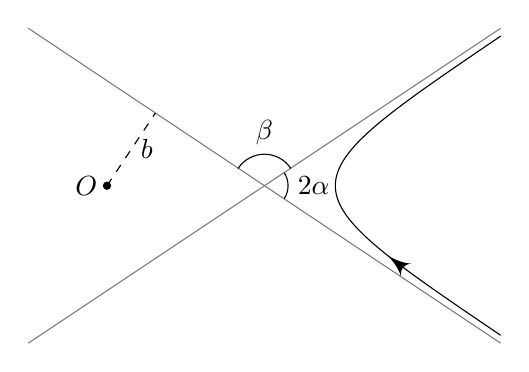
\begin{tikzpicture}
    \draw [gray] (-3, -2) -- (3, 2);
    \draw [gray] (3, -2) -- (-3, 2);
    \draw [->-=0.3] (3, -1.9) .. controls (0.2, 0) .. (3, 1.9);
    \node at (-2, 0) [circ] {};
    \node at (-2, 0) [left] {$O$};
    \draw [dashed] (-2, 0) -- (-1.38462, 0.923077) node [pos = 0.5, right] {$b$};
    \draw (0.3, 0) arc (0:-33:0.3);
    \draw (0.3, 0) arc (0:33:0.3);
    \node at (0.3, 0) [right] {$2\alpha$};
    \draw (0, 0.4) arc (90:33:0.4);
    \draw (0, 0.4) arc (90:147:0.4);
    \node at (0, 0.4) [above] {$\beta$};
  \end{tikzpicture}
\end{center}
It seems as if the particle is deflected by $O$.

Far from the origin, the orbit tends towards uniform motion with speed $v$ in a straight line. Then angular momentum per unit mass is $h = bv$ (velocity $\times$ perpendicular distance to $O$.

How does the scattering angle $\beta = \pi = 2\alpha$ depend on the impact parameter $b$ and the incident speed $v$?

From the above,
\[
  \frac{1}{e} = \cos \alpha = \cos \left(\frac{\pi}{2} - \frac{\beta}{2}\right) = \sin\left(\frac{\beta}{2}\right),
\]
So
\[
  b = \frac{\ell}{\sqrt{e^2 - 1}} = \frac{(bv)^2}{k}\tan \frac{\beta}{2}.
\]
So
\[
  \beta = 2\tan^{-1}\left(\frac{k}{bv^2}\right).
\]

So scattering angles approach $\pi$ can be obtained for small impact parameters, $b \ll k/v^2$.

\section{Rotating frames}
\begin{center}
  \includegraphics[scale=0.75]{images/xkcd_centrifugal_force.png}\\
  xkcd (Randall Munroe) CC-BY-NC 2.5
\end{center}
Newton's laws hold only in inertial frames. A rotating frame is not inertial and the equation of motion is modified.

Let $S$ be an inertial frame, and let $S'$ be a non-inertial frame, rotating about the $z$ axis with angular velocity $\omega = \dot{\theta}$ with respect to $S$.

Call the basis vectors $\mathbf{e}_i = \{\hat{\mathbf{x}}, \hat{\mathbf{y}}, \hat{\mathbf{z}}\}$ and $\mathbf{e}_i' = \{\hat{\mathbf{x}}', \hat{\mathbf{y}}', \hat{\mathbf{z}}'\}$.

Consider a particle at rest in $\mathbf{S}'$. From the perspective of $S$, its velocity is
\[
  \left(\frac{\d \mathbf{r}}{\d t}\right)_S = \boldsymbol\omega\times \mathbf{r},
\]
where $\boldsymbol\omega = \omega\hat{\mathbf{z}}$ is the \emph{angular velocity vector} (aligned with the rotation axis). This formula also applies to the basis vectors of $S'$.
\[
  \left(\frac{\d \mathbf{e}_i'}{\d t}\right)_S = \boldsymbol\omega\times \mathbf{e}_i'.
\]
A general time-dependent vector $\mathbf{a}$ can be written as
\[
  \mathbf{a} = \sum a_i'(t) \mathbf{e}_i'.
\]
From the perspective of $S'$, with $\mathbf{e}_i'$ constant and its time derivative is
\[
  \left(\frac{\d \mathbf{a}}{\d t}\right)_{S'} = \sum \frac{\d a_i'}{\d t}\mathbf{e}_i'.
\]
In $S$, however, $\mathbf{e}_i'$ is not constant, and its time derivative is
\[
  \left(\frac{\d \mathbf{a}}{\d t}\right)_S = \sum \frac{\d a_i}{\d t}\mathbf{e}_i' + \sum a_i'\boldsymbol\omega \times \mathbf{e}_i' = \left(\frac{\d \mathbf{a}}{\d t}\right)_{S'} + \boldsymbol\omega \times \mathbf{a}.
\]
This key identity applies to all vectors and can be written as an operator equation:
\begin{prop}
  If $S$ is an inertial frame, and $S'$ is rotating relative to $S$ with angular velocity $\boldsymbol \omega$, 
  \[
    \left(\frac{\d}{\d t}\right)_S = \left(\frac{\d}{\d t}\right)_{S'} + \boldsymbol\omega \times.
  \]
  Applied to the position vector $\mathbf{r}(t)$ of a particle, it gives
  \[
    \left(\frac{\d \mathbf{r}}{\d t}\right)_S = \left(\frac{\d \mathbf{r}}{\d t}\right)_{S'} + \boldsymbol\omega \times \mathbf{r}.
  \]
\end{prop}
So the difference in velocity measured in the two frames is the relative velocity of the frames, which depends on position.

Applied a second time, and allowing for $\boldsymbol\omega$ to depend on time, it gives
\begin{align*}
  \left(\frac{\d ^2\mathbf{r}}{\d t^2}\right)_S &= \left(\left(\frac{\d }{\d t}\right)_{S'} + \boldsymbol\omega\times \right)\left(\left(\frac{\d \mathbf{r}}{\d t}\right)_{S'} + \boldsymbol\omega \times \mathbf{r}\right).\\
  &= \left(\frac{\d^2 \mathbf{r}}{\d t^2}\right)_{S'} + 2\boldsymbol \omega \times \left(\frac{\d \mathbf{r}}{\d t}\right)_{S'} + \dot{\boldsymbol\omega} \times \mathbf{r} + \boldsymbol\omega\times(\boldsymbol\omega\times \mathbf{r})
\end{align*}
Since $S$ is inertial, Newton's Second Law is
\[
  m\left(\frac{\d ^2\mathbf{r}}{\d t^2}\right)_S = \mathbf{F}.
\]
So
\begin{prop}
  \[
    m\left(\frac{\d^2 \mathbf{r}}{\d t^2}\right) = \mathbf{F} - 2m\boldsymbol\omega \times \left(\frac{\d \mathbf{r}}{\d t}\right)_{S'} - m\dot{\boldsymbol\omega}\times \mathbf{r} - m\boldsymbol\omega \times (\boldsymbol\omega \times \mathbf{r}).
  \]
\end{prop}

\begin{defi}[Fictious forces]
  The additional terms on the RHS of the equation of motion in rotating frames are \emph{fictitious forces}, and are needed to explain the motion observed in $S'$. They are
  \begin{itemize}
    \item \emph{Coriolis force}: $-2m\boldsymbol\omega \times \left(\frac{\d \mathbf{r}}{\d t}\right)_{S'}.$
    \item \emph{Euler force}: $-m\dot{\boldsymbol\omega}\times \mathbf{r}$
    \item \emph{Centrifugal force}: $-m\boldsymbol\omega\times(\boldsymbol\omega\times \mathbf{r})$.
  \end{itemize}
\end{defi}
Usually we consider $\boldsymbol \omega$ to be constant and can neglect the Euler force.

A frame fixed to the Earth rotates with angular velocity
\[
  \omega = \frac{2\pi}{1\text{ day}} \approx \SI{7.3e-5}{\per\second}.
\]
\subsection{The centrifugal force}
Let $\boldsymbol\omega = \omega\hat{\boldsymbol\omega}$, where $|\hat{\boldsymbol\omega}| = 1$. Then
\[
  -m\boldsymbol\omega \times (\boldsymbol\omega \times \mathbf{r}) = -m\big((\boldsymbol\omega \cdot \mathbf{r})\boldsymbol\omega - (\boldsymbol\omega \cdot \boldsymbol\omega)\mathbf{r}\big) = m\omega^2 \mathbf{r}_{\bot},
\]
where $\mathbf{r}_{\bot} = \mathbf{r} - (\mathbf{r}\cdot \hat{\boldsymbol\omega})\hat{\boldsymbol\omega}$, the projection of the position on the plane perpendicular to $\boldsymbol\omega$. So the centrifugal force is directed away from the axis of rotation and its magnitude is $m\omega^2$ times the distance form the axis.

\begin{center}
  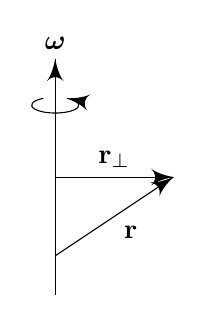
\begin{tikzpicture}
    \draw [->] (0, 0) -- (0, 3) node [above] {$\boldsymbol\omega$};
    \draw [->] (-0.15, 2.5) arc (120:420:0.3 and 0.1);
    \draw [->] (0, 0.5) -- (1.5, 1.5) node [pos=0.5, anchor = north west] {$\mathbf{r}$};
    \draw [->] (0, 1.5) -- (1.5, 1.5) node [pos = 0.5, above] {$\mathbf{r}_\bot$};
  \end{tikzpicture}
\end{center}
Note that
\begin{align*}
  \mathbf{r}_\bot \cdot \mathbf{r}_\bot &= \mathbf{r}\cdot \mathbf{r} - (\mathbf{r} \cdot \hat{\boldsymbol\omega})^2\\
  \nabla(|\mathbf{r}_\bot|^2) &= 2\mathbf{r} - 2(\mathbf{r}\cdot \hat{\boldsymbol\omega})\hat{\boldsymbol\omega} = 2\mathbf{r}_\bot.
\end{align*}
So
\[
  -m\boldsymbol\omega\times(\boldsymbol\omega\times \mathbf{r}) = -\nabla\left(-\frac{1}{2}m\omega^2|\mathbf{r}_\bot|^2\right) = -\nabla\left(-\frac{1}{2}m|\boldsymbol\omega\times \mathbf{r}|^2\right).
\]
On a rotating planet, the gravitational and centrifugal forces per unit mass combine to make the \emph{effective gravity},
\[
  \mathbf{g}_{\text{eff}} = \mathbf{g} + \omega^2 \mathbf{r}_\bot.
\]
This gravity will not be vertically downwards. Consider a point $P$ at latitude $\lambda$ on the surface of a spherical planet of radius $R$.

We construct orthogonal axes:
\begin{center}
  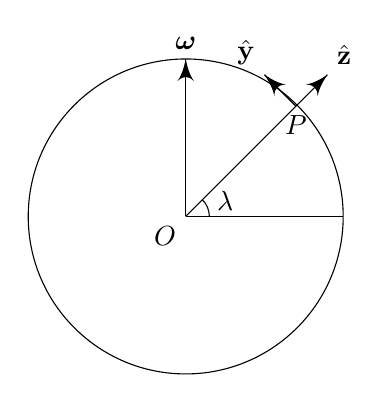
\begin{tikzpicture}
    \draw circle [radius = 2];
    \node [anchor = north east] {$O$};
    \draw [->] (0, 0) -- (0, 2) node [above] {$\boldsymbol\omega$};
    \draw (0, 0) -- (2, 0);
    \draw (0, 0) -- (1.4, 1.4) node [below] {$P$};
    \draw [->] (1.4, 1.4) -- (1.8, 1.8) node [anchor = south west] {$\hat{\mathbf{z}}$};
    \draw [->] (1.4, 1.4) -- (1, 1.8) node [anchor = south east] {$\hat{\mathbf{y}}$};
    \draw (0.3, 0) arc (0:45:0.3);
    \node at (0.5, 0.2) {$\lambda$};
  \end{tikzpicture}
\end{center}
with $\hat{\mathbf{x}}$ into the page. So $\hat{\mathbf{z}}$ is up, $\hat{\mathbf{y}}$ is North, and $\hat{\mathbf{x}}$ is East.

At $P$, we have
\begin{align*}
  \mathbf{r} &= R\hat{\mathbf{z}}\\
  \mathbf{g} &= -g\hat{\mathbf{z}}\\
  \boldsymbol\omega &= \omega(\cos\lambda \hat{\mathbf{y}} + \sin \lambda \hat{\mathbf{z}})
\end{align*}
So
\begin{align*}
  \mathbf{g}_{\mathrm{eff}} &= \mathbf{g} + \omega^2 \mathbf{r}_\bot \\
  &= -g\hat{\mathbf{z}} + \omega^2 R\cos\lambda(\cos\lambda\hat{\mathbf{z}} - \sin\lambda\hat{\mathbf{y}})\\
  &= -\omega^2 R\cos\lambda\sin\lambda\hat{\mathbf{y}} - (g - \omega^2 R\cos^2\lambda)\hat{\mathbf{z}}.
\end{align*}
So the angle $\alpha$ between $\mathbf{g}$ and $\mathbf{g}_{\text{eff}}$ is given by
\[
  \tan \alpha = \frac{\omega^2 R\cos\lambda\sin\lambda}{g - \omega^2R\cos^2\lambda}.
\]
This is 0 at the equator and the poles, and greatest when you are halfway between. However, this is still tiny on Earth, and does not affect our daily life.

\subsection{The Coriolis force}
This depends on the velocity in the rotating frame, $\mathbf{v} = \left(\frac{\d \mathbf{r}}{\d t}\right)_{S'}$:
\[
  \mathbf{F} = -2m\boldsymbol\omega\times \mathbf{v},
\]
like the Lorentz force on a charged particle in a magnetic field. However, this does not mean that particles will go around in circles, as in the case of magnetic fields, since we also have the centrifugal force in play.

Since this is always perpendicular to the velocity, it does no work.

Consider potion parallel to the Earth's surface. We only care about the effect of the Coriolis force on the horizontal trajectory, and ignore the vertical component that is tiny compared to gravity.

So we only take the vertical component of $\boldsymbol\omega$, $\omega\sin\lambda\hat{\mathbf{z}}$. The horizontal velocity $\mathbf{v} = v_x \hat{\mathbf{x}} + v_y \hat{\mathbf{y}}$ generates a horizontal Coriolis force:
\[
  -2m\omega\sin\lambda\hat{\mathbf{z}}\times \mathbf{v} = -2m\omega\sin\lambda(v_y \hat{\mathbf{x}} - v_x \hat{\mathbf{y}}).
\]
In the Northern hemisphere $(0 < \lambda < \pi/2)$, this causes a deflection towards the right. In the Southern Hemisphere, the deflection is to the left. The effect vanishes at the equator.

\note Only the horizontal effect on horizontal motion vanishes at the equator. The vertical effects or those caused by vertical motion still exist.

\begin{eg}
  Suppose a ball is dropped from a tower of height $h$ at the equator. Where does it land?

  In the rotating frame,
  \[
    \dot{\mathbf{r}} = \mathbf{g} - 2\boldsymbol\omega\times \dot{\mathbf{r}} - \boldsymbol\omega\times(\boldsymbol\omega\times \mathbf{r}).
  \]
  We work to first order in $\omega$. Then
  \[
    \dot{\mathbf{r}} - 2\boldsymbol\omega\times \dot{\mathbf{r}} + O(\omega^2).
  \]
  Integrate wrt $t$ to obtain
  \[
    \dot{\mathbf{r}} = \mathbf{g}t - 2\boldsymbol\omega \times (\mathbf{r} - \mathbf{r}_0) + O(\omega^2),
  \]
  where $\mathbf{r}_0$ is the initial position. We substitute into the original equation to obtain
  \[
    \dot{\mathbf{r}} = \mathbf{g}\boldsymbol\omega\times \mathbf{g}t + O(\omega^2).
  \]
  (where some new $\omega^2$ terms are thrown into $O(\omega^2)$). We integrate twice to obtain
  \[
    \mathbf{r} = \mathbf{r}_0 + \frac{1}{2}\mathbf{g}t^2 - \frac{1}{3}\boldsymbol\omega \times \mathbf{g}t^3 + O(\omega^2).
  \]
  In components, where $\mathbf{g} = (0, 0, -g)$, $\boldsymbol\omega = (0, \omega, 0)$, and $\mathbf{r}_0 = (0, 0, R + h)$. So
  \[
    \mathbf{r} = \left(\frac{1}{3}\omega gt^3, 0, R + h - \frac{1}{2}gt^2\right) + O(\omega^2).
  \]

  So the particle hits the ground at $t = \sqrt{2h/g}$, and its eastward displacement is $\frac{1}{3}wg\left(\frac{2h}{g}\right)^{3/2}$.

  This can be understood in terms of angular momentum conservation in the non-rotating frame. At the beginning, the particle has the same angular velocity with the Earth. As it falls towards the Earth, to maintain the same angular momentum, the angular velocity has to increase to compensate for the decreased radius. So it spins faster than the Earth and drifts towards the East, relative to the Earth.
\end{eg}

\begin{eg}
  Consider a pendulum that is free to swing in any plane, eg. a weight on a string. At the North pole, it will swing in a plane that is fixed in an inertial frame, while the Earth rotates beneath it. From the perspective of the rotating frame, the plane of the pendulum rotates backwards. This can be explained as a result of the Coriolis force.

  At latitude $\lambda$, the plane rotates with period $\frac{1\text{ day}}{\sin \lambda}$ (the Coriolis force makes the particle deflect to the right. So the plane with keep turning rightwards as well).
\end{eg}

\section{Systems of particles}
Consider a system of $N$ interacting particles. Particle $i$ has mass $m_i$, position $\mathbf{r}_i$, and momentum $\mathbf{p}_i = m_i \dot{\mathbf{r}}_i$. Note that the subscript denotes which particle it is referring to, not vector components.

Newton's Second Law for particle $i$ is
\[
  m_i \ddot{\mathbf{r}}_i = \dot{\mathbf{p}}_i = \mathbf{F}_i,
\]
where
\[
  \mathbf{F}_i = \mathbf{F}_i^{\text{ext}} = \sum_{j = 1}^N \mathbf{F}_{ij},
\]
where $\mathbf{F}_{ij}$ is the force on particle $i$ by particle $j$, and $\mathbf{F}_i^{\text{ext}}$ is the external force on $i$, which comes from particles outside the system.

Since a particle cannot exert a force on itself, so $\mathbf{F}_{ii} = \mathbf{0}$. Also, Newton's third law requires that
\[
  \mathbf{F}_{ij} = -\mathbf{F}_{ji}.
\]
If we represent the forces as a matrix, then the matrix is antisymmetric.

For example, for gravitational forces,
\[
  \mathbf{F}_{ij} = -\frac{Gm_im_j(\mathbf{r}_i - \mathbf{r}_j)}{|\mathbf{r}_i - \mathbf{r}_j|^3} = -\mathbf{F}_{ji}.
\]
\subsection{Motion of the center of mass}
\begin{defi}[Total mass]
  The \emph{total mass} of the system is $M = \sum m_i$.
\end{defi}

\begin{defi}[Center of mass]
  The \emph{center of mass} is located at
  \[
    \mathbf{R} = \frac{1}{M}\sum_{i = 1}^N m_i\mathbf{r}_i,
  \]
  ie. the mass-weighted average position.
\end{defi}

\begin{defi}[Total linear momentum]
  The \emph{total linear momentum} is
  \[
    \mathbf{P} = \sum_{i = 1}^N \mathbf{p}_i = \sum_{i = 1}^N m_i \dot{\mathbf{r}}_i = M\dot{\mathbf{R}}.
  \]
  This is equivalent to that of a single particle of mass $M$ at the center of mass.
\end{defi}

\begin{defi}[Total external force]
  The \emph{total external force} is
  \[
    \mathbf{F} = \sum_{i = 1}^N \mathbf{F}_i^{\text{ext}}.
  \]
\end{defi}
Then
\begin{prop}
  \[
    M\ddot{\mathbf{R}} = \mathbf{F}.
  \]
\end{prop}

\begin{proof}
\begin{align*}
  M\ddot{\mathbf{R}} &= \dot{\mathbf{P}}\\
  &= \sum_{i = 1}^N \dot{\mathbf{p}}_i\\
  &= \sum_{i = 1}^N \mathbf{F}_i^{\text{ext}} + \sum_{i = 1}^N\sum_{j = 1}^N \mathbf{F}_{ij}\\
  &= \mathbf{F} + \frac{1}{2}\sum_i \sum_j(\mathbf{F}_{ij} + \mathbf{F}_{ji})\\
  &= \mathbf{F}
\end{align*}
\end{proof}
So the center of mass moves as a particle of mass $M$ subject to a force $\mathbf{F}$. This is why Newton's Laws apply to macroscopic objects even though they are not individual particles.

\begin{law}[Conservation of momentum]
  If $\mathbf{F} = \mathbf{0}$, then $\dot{\mathbf{P}} = \mathbf{0}$. So the total momentum is conserved.
\end{law}

\begin{defi}[Center of mass frame]
  The \emph{center of mass frame} is an inertial frame in which $\mathbf{R} = 0$ for all time.
\end{defi}

\begin{defi}[Total angular momentum]
  The \emph{total angular momentum} of the system about the origin is
  \[
    \mathbf{L} = \sum_i  \mathbf{r}_i \times \mathbf{p}_i.
  \]
\end{defi}

So
\begin{align*}
  \dot{\mathbf{L}} &= \sum_i \mathbf{r}_i \times \dot{\mathbf{p}}_i + \dot{\mathbf{r}}_i \times \mathbf{p}_i\\
  &= \sum  \mathbf{r}_i\times \dot{\mathbf{p}}_i\\
  &= \sum_i \mathbf{r}_i\times \mathbf{F}_i^{\text{ext}} + \sum_i \sum_j \mathbf{r}_i \times \mathbf{F}_{ij}\\
  &= \sum_i \mathbf{G}_i^{\text{ext}} + \frac{1}{2}\sum_i\sum_j (\mathbf{r}_i \times \mathbf{F}_{ij} + \mathbf{r}_j\times \mathbf{F}_{ji})\\
  &= \mathbf{G} + \frac{1}{2}\sum_i\sum_j(\mathbf{r}_i - \mathbf{r}_j)\times \mathbf{F}_{ij}\\
  \intertext{Usually the second sum is zero (see later), and we have}\\
  &= \mathbf{G},
\end{align*}
where
\begin{defi}[Total external torque]
  The \emph{total external torque} is
  \[
    \mathbf{G} = \sum_i \mathbf{r}_i \times \mathbf{F}_i^{\text{ext}}.
  \]
\end{defi}
The last line holds provided the ``strong version'' of Newton's Third Law holds:
\[
  \mathbf{F}_{ij} = -\mathbf{F}_{ji}\text{ and is parallel to }(\mathbf{r}_i - \mathbf{r}_j).
\]
This is true, at least, for gravitational and electrostatic forces. So the total angular momentum is conserved if $\mathbf{G} = \mathbf{0}$, ie the total external torque vanishes.

\subsection{Motion relative to the center of mass}
Let $\mathbf{r}_i = \mathbf{R} + \mathbf{r}_i^c$, where $\mathbf{r}_i^c$ is the position of particle $i$ relative to the center of mass.

Then
\[
  \sum_i m_i\mathbf{r}_i^c = \sum m_i \mathbf{r}_i - \sum m_i \mathbf{R} = M\mathbf{R} - M\mathbf{R} = \mathbf{0}.
\]
Also,
\[
  \sum_i m_i \dot{\mathbf{r}}_i^c = \mathbf{0}.
\]
Using the equalities above, we can express the total linear momentum, angular momentum and kinetic energy in terms of $\mathbf{R}$ and $\mathbf{r}_i^c$ only:
\begin{align*}
  \mathbf{P} &= \sum_i m_i(\dot{\mathbf{R}} + \dot{\mathbf{r}}_i^c) = M\dot{\mathbf{R}}\\
  \mathbf{L} &= \sum_i m_i(\mathbf{R} + \mathbf{r}_i^c) \times (\dot{\mathbf{R}} + \dot{\mathbf{r}}_i^c)\\
  &= \sum_i m_i \mathbf{R}\times \dot{\mathbf{R}} + \mathbf{R}\times \sum_i m_i \dot{\mathbf{r}}_i^c + \sum_i m_i \mathbf{r}_i^c\times \dot{\mathbf{R}} + \sum_i m_i \mathbf{r}_i^c \times \dot{\mathbf{r}}_i^c\\
  &= M\mathbf{R}\times \dot{\mathbf{R}} + \sum_i m_i \mathbf{r}_i^c \times \dot{\mathbf{r}}_i^c\\
  T&= \frac{1}{2}\sum_i m_i|\dot{\mathbf{r}}_i|^2\\
  &= \frac{1}{2}\sum_i m_I (\dot{\mathbf{R}} + \dot{\mathbf{r}_i}^c)\cdot (\dot{\mathbf{R}} + \dot{\mathbf{r}}_i^c)\\
  &= \frac{1}{2}\sum_i m_i \dot{\mathbf{R}}\cdot \dot{\mathbf{R}} + \dot{\mathbf{R}} \cdot \sum_i m_i \dot{\mathbf{r}}_i^c + \frac{1}{2}\sum_i m_i \dot{\mathbf{r}}_i^c\cdot \dot{\mathbf{r}}_i^c\cdot \dot{\mathbf{r}}_i^c\\
  &=\frac{1}{2}M|\dot{\mathbf{R}}|^2 + \frac{1}{2}\sum_i m_i|\dot{\mathbf{r}}_i^c|^2
\end{align*}
In the case of the angular momentum and the kinetic energy, we see that they are composed of two parts - that of the center of mass and that of motion relative to center of mass.

If the forces are conservative in the sense that
\[
  \mathbf{F}_i^{\text{ext}} = -\nabla_i V_i(\mathbf{r}_i),
\]
and
\[
  \mathbf{F}_{ij} = -\nabla_i V_{ij} (\mathbf{r}_i - \mathbf{r}_j),
\]
where $\nabla_i$ is the gradient with respect to $\mathbf{r}_i$, then energy is conserved in the from
\[
  E = T + \sum_i V_i(\mathbf{r}_i) + \frac{1}{2}\sum_i\sum_j V_{ij}(\mathbf{r}_i - \mathbf{r}_j) = \text{const.}
\]
\subsection{The two-body problem}
Consider two particles with no external forces. The center of mass is at
\[
  \mathbf{R} = \frac{1}{M} (m_i \mathbf{r}_i + m_2 \mathbf{r}_2),
\]
where $M = m_1 + m_2$.

Define the separation vector (or relative position vector)
\[
  \mathbf{r} = \mathbf{r}_1 - \mathbf{r}_2.
\]
Then
\[
  \mathbf{r}_1 = \mathbf{R} + \frac{m_2}{M}\mathbf{r},\quad \mathbf{r}_2 = \mathbf{R} - \frac{m_1}{M}\mathbf{r}.
\]
\begin{center}
  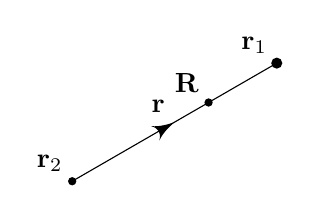
\begin{tikzpicture}[rotate=30]
    \node [circ] {};
    \node [anchor = south east] {$\mathbf{r}_2$};

    \node at (3, 0) [circ, minimum size = 4] {};
    \node at (3, 0) [anchor = south east] {$\mathbf{r}_1$};

    \node at (2, 0) [circ, minimum size = 3] {};
    \node at (2, 0) [anchor = south east] {$\mathbf{R}$};
    \draw [->-=0.5] (0, 0) -- (3, 0) node [pos =0.5, anchor = south east] {$\mathbf{r}$};
  \end{tikzpicture}
\end{center}

Since $\mathbf{F} = \mathbf{0}$, $\ddot{\mathbf{R}} = \mathbf{0}$, ie. the center of mass moves uniformly.

Meanwhile,
\begin{align*}
  \ddot{\mathbf{r}} &= \ddot{\mathbf{r}}_1 - \ddot{\mathbf{r}}_2\\
  &= \frac{1}{m_1} \mathbf{F}_{12} - \frac{1}{m_2}\mathbf{F}_{21}\\
  &= \left(\frac{1}{m_1} + \frac{1}{m_2}\right) \mathbf{F}_{12}\\
\end{align*}
We can write this as
\[
  \mu \ddot{\mathbf{r}} = \mathbf{F}_{12}(\mathbf{r}),
\]
where
\[
  \mu = \frac{m_1m_2}{m_1 + m_2}
\]
is the \emph{reduced mass}. This is the same as the equation of motion for \emph{one particle} of mass $\mu$ with position vector $\mathbf{r}$ relative to a fixed origin - as studied previously.

For example, with gravity,
\[
  \mu \ddot{\mathbf{r}} = -\frac{Gm_1m_2 \hat{\mathbf{r}}}{|\mathbf{r}|^2}.
\]
So
\[
  \ddot{\mathbf{r}} = -\frac{GM\hat{\mathbf{r}}}{|\mathbf{r}|^2}.
\]
For example, give a planet orbiting the Sun, both the planet and the sun moves in ellipses about their center of mass. The orbital period depends on the total mass.

It can be shown that
\begin{align*}
  \mathbf{L} &= M\mathbf{R} \times \dot{\mathbf{R}} + \mu \mathbf{r}\times \dot{\mathbf{r}}\\
  T &= \frac{1}{2} M|\dot{\mathbf{R}}|^2 + \frac{1}{2}\mu |\dot{\mathbf{r}}|^2.
\end{align*}

\subsection{Variable-mass problem}
Rockets, fireworks, falling raindrops, rolling snowballs, are all objects whose mass decreases or increases with time.

Newton's second law is
\[
  \frac{\d \mathbf{p}}{\d t} = \mathbf{F},\quad\text{with }\mathbf{p} = m\dot{\mathbf{r}}.
\]
But we cannot simply apply this with $m = m(t)$, because these systems are not closed.

Consider a rocket moving in one dimension with mass $m(t)$ and velocity $v(t)$. The rocket propels itself forwards by burning fuel and ejecting the exhaust at velocity $-u$ relative to the rocket.

At time $t$: 
\begin{center}
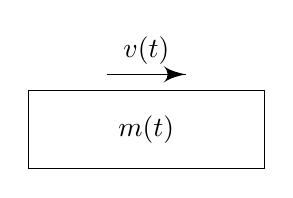
\begin{tikzpicture}
  \draw (0, 0.5) rectangle (3, -0.5);
  \node at (1.5, 0) {$m(t)$};
  \draw [->] (1, 0.7) -- (2, 0.7) node [pos = 0.5, above] {$v(t)$};
\end{tikzpicture}
\end{center}
At time $t + \delta t$, it ejects exhaust of mass $m(t) - m(t + \delta t)$ with velocity $v(t) - u + O(\delta t)$.

\begin{center}
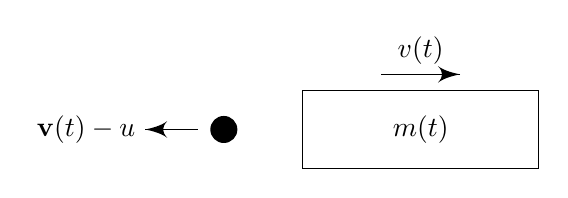
\begin{tikzpicture}
  \draw (0, 0.5) rectangle (3, -0.5);
  \node at (1.5, 0) {$m(t)$};
  \draw [->] (1, 0.7) -- (2, 0.7) node [pos = 0.5, above] {$v(t)$};
  \node at (-1, 0) [circ] {$m$};
  \draw [->] (-1.33, 0) -- (-2, 0) node [left] {$\mathbf{v}(t) - u$};
\end{tikzpicture}
\end{center}

The change in total momentum of the system (rocket + exhaust) is
\begin{align*}
  \delta p &= m(t + \delta t)v(t + \delta t) + [m(t) - m(t + \delta t)][v(t) - u(t) + O(\delta t)] - m(t)v(t)\\
  &= (m + \dot{m}\delta t + O(\delta t^2))(v + \dot{v} \delta t + O(\delta t^2)) - \dot{m}\delta t(v - u) + O(\delta t^2) - mv\\
  &= (\dot{m}v + m\dot{v} - \dot{m}v + \dot{m}u)\delta t + O(\delta t^2)\\
  &= (m\dot{v} + \dot{m}u)\delta t + O(\delta t^2).
\end{align*}
Newton's second law gives
\[
  \lim_{\delta \to 0} \frac{\delta p}{\delta t} = F\text{ (the external force on rocket)}
\]
So
\begin{prop}[Rocket equation]
  \[
    m\frac{\d v}{\d t} + u\frac{\d m}{\d t} = F.
  \]
\end{prop}
\begin{eg}
  When $F = 0$ (and $u$ is constant), we have
  \[
    m\frac{\d v}{\d t} = -u\frac{\d m}{d t}.
  \]
  So
  \[
    v = v_0 + u \log \left(\frac{m_0}{m(t)}\right),
  \]
  Note that are expressing things in terms of the mass remaining $m$, not time $t$.

  Note also that the velocity does not depend on the rate at which mass is ejected, only the velocity at which it is ejected.
\end{eg}

\begin{eg}
  Consider a falling raindrop of mass $m(t)$, gathering mass from a stationary cloud. In this case, $u = v$. So
  \[
    m\frac{\d v}{\d t} + v\frac{\d m}{\d t} = \frac{\d }{\d t}(mv) = mg,
  \]
  with $v$ measured downwards. To solve this, we need a model to determine the rate at which the raindrop gathers mass.
\end{eg}

\section{Rigid bodies}
\begin{defi}[Rigid body]
  A \emph{rigid body} is an extended object, consisting of $N$ particles that are constrained such that the distance between any pair of particles, $|\mathbf{r}_i - \mathbf{r}_j|$, is fixed.
\end{defi}
Intuitively, it is a solid object that cannot deform.

The possible motions of a rigid body are the continuous isometries of Euclidean space, ie. translations and rotations.
\subsection{Angular velocity}
Consider a single particle moving in a circle of radius $s$ about the $z$ axis. Its position and velocity vectors are
\begin{align*}
  \mathbf{r} &= (s\cos \theta, s\sin \theta, z)\\
  \dot{\mathbf{r}} &= (-s \dot{\theta}\sin \theta, s\dot{\theta}\cos \theta, 0).
\end{align*}
We can write
\[
  \dot{\mathbf{r}} = \boldsymbol\omega\times \mathbf{r},
\]
where
\[
  \boldsymbol\omega = \dot{\theta}\hat{\mathbf{z}}
\]
is the angular velocity vector.

In general,
\[
  \boldsymbol\omega = \dot{\theta} \hat{\mathbf{n}} = \omega\hat{\mathbf{n}},
\]
where $\hat{\mathbf{n}}$ is a unit vector parallel to the rotation axis.

The kinetic energy of this particle is
\begin{align*}
  T &= \frac{1}{2}m|\dot{\mathbf{r}}|^2\\
  &= \frac{1}{2}m s^2 \dot{\theta}^2\\
  &= \frac{1}{2}I \omega^2
\end{align*}
where $I$ is the \emph{moment of inertia}. This is the counterpart of ``mass'' in rotational motion (cf. $\frac{1}{2}mv^2$ vs $\frac{1}{2}I\omega^2$).
\begin{defi}[Moment of inertia]
  The \emph{moment of inertia} of a particle is
  \[
    I = ms^2 = m|\hat{\mathbf{n}}\times \mathbf{r}|^2,
  \]
  where $s$ is the distance of the particle from the axis of rotation.
\end{defi}
\subsection{Moment of inertia}
Consider a rigid body in which all $N$ particles rotate about the same axis with the same angular velocity:
\[
  \dot{\mathbf{r}}_i = \boldsymbol\omega\times \mathbf{r}_i.
\]
This ensures that
\[
  \frac{\d }{\d t}|\mathbf{r}_i - \mathbf{r}_j|^2 = 2(\dot{\mathbf{r}}_i - \dot{\mathbf{r}}_j)\cdot (\mathbf{r}_i - \mathbf{r}_j) = 2\big(\boldsymbol\omega\times (\mathbf{r}_i - \mathbf{r}_j)\big) \cdot (\mathbf{r}_i - \mathbf{r}_j) = 0,
\]
as required for a rigid body.

The rotational kinetic energy is
\[
  T = \frac{1}{2}\sum_{i = 1}^N m_i|\dot{\mathbf{r}_i}|^2 = \frac{1}{2}I\omega^2,
\]
where
\begin{defi}[Moment of inertia]
  The \emph{moment of inertia} of a rigid body about the rotation axis $\hat{\mathbf{n}}$ is
  \[
    I = \sum_{i = 1}^N m_is_i^2 = \sum_{i = 1}^N m_i |\hat{\mathbf{n}}\times \mathbf{r}_i|^2.
  \]
\end{defi}
\begin{defi}
  The angular momentum is
  \[
    \mathbf{L} = \sum_i m_i \mathbf{r}_i \times \dot{\mathbf{r}}_i = \sum_i m_i \mathbf{r}_i \times (\boldsymbol\omega \times \mathbf{r}_i).
  \]
\end{defi}
If we write 
\[
  \boldsymbol\omega = \omega\hat{\mathbf{n}},
\]
then the component of $\mathbf{L}$ in the direction of $\hat{\mathbf{n}}$ is
\begin{align*}
  \mathbf{L} \cdot \hat{\mathbf{n}} &= \omega \sum_i m_i \hat{\mathbf{n}}\cdot (\mathbf{r}_i \times (\hat{\mathbf{n}} \times \mathbf{r}_i))\\
  &= \omega \sum_i m(\hat{\mathbf{n}}\times \mathbf{r}_i)\cdot (\hat{\mathbf{n}} \times \mathbf{r}_i)\\
  &= I\omega
\end{align*}
However, $\mathbf{L}$ may not be parallel to to $\boldsymbol\omega$ in general. Using vector identities, we have
\[
  \mathbf{L} = \sum_i m_i\big((\mathbf{r}_i\cdot \mathbf{r}_i)\boldsymbol \omega - (\mathbf{r}_i \cdot \boldsymbol\omega)\mathbf{r}_i\big)
\]
Note that this is a linear function of $\boldsymbol\omega$. So we can write
\[
  \mathbf{L} = I\boldsymbol \omega
\]
where $I$ is the \emph{inertia tensor} represented by a symmetric matrix with components
\[
  I_{jk} = \sum_i m_i(|\mathbf{r}_i|^2 \delta_{jk} - (\mathbf{r}_i)_j(\mathbf{r}_i)_k),
\]
where $i$ refers to the index of the particle, and $j, k$ and dummy suffixes summed over.

If the body rotates about a \emph{principal axis}, ie. one of the three orthogonal eigenvectors of $I$, (eg. an axis of rotational symmetry if the body has one), then $\mathbf{L}$ is parallel to $\boldsymbol\omega$.

The relations $T = \frac{1}{2}I\omega^2$ and $L = I\omega$ for angular motion are analogous to the relations $T = \frac{1}{2}mv^2$ and $p = mv$ for linear motion.

\subsection{Calculating the moment of inertia}
For a solid body, we usually want to think of it as a continuous substance with a mass density, instead of individual point particles. So we replace the sum of particles by a volume integral weighted by the mass density $\rho(\mathbf{r})$.

\begin{defi}[Mass, center of mass and moment of inertia]
  The \emph{mass} is
  \[
    M = \int \rho \;\d V.
  \]
  The \emph{center of mass} is
  \[
    \mathbf{R} = \frac{1}{M}\int \rho  \mathbf{r}\;\d V
  \]
  The \emph{moment of inertial}is
  \[
    I = \int \rho s^2 \;\d V = \int \rho|\hat{\mathbf{n}}\times \mathbf{r}|^2\;\d V.
  \]
\end{defi}
In theory, we can study inhomogeneous bodies with varying $\rho$, but usually we mainly consider homogeneous ones with constant $\rho$ throughout.

\begin{eg}[Thin circular ring]
  Suppose the ring has mass $M$ and radius $a$, and a rotation axis through the center, perpendicular to the plane of the ring.
  \begin{center}
    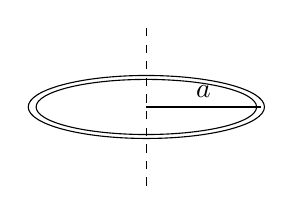
\begin{tikzpicture}
      \draw circle [x radius = 1.5, y radius = 0.4];
      \draw circle [x radius = 1.4, y radius = 0.35];
      \draw (0, 0) -- (1.45, 0) node [pos = 0.5, above] {$a$};
      \draw [dashed] (0, -1) -- (0, 1);
    \end{tikzpicture}
  \end{center}
  Then the moment of inertia is
  \[
    I = Ma^2.
  \]
\end{eg}

\begin{eg}[Thin rod]
  Suppose a rod has mass $M$ and length $\ell$. It rotates through one end, perpendicular to the rod.
 
  \begin{center}
    \begin{tikzpicture}
      \draw [dashed] (0, -1) -- (0, 1);
      \draw (0, 0.05) rectangle (2, -0.05);
      \node at (1, 0.3) {$\ell$};
    \end{tikzpicture}
  \end{center}
  The mass per unit length is $M/\ell$. So the moment of inertia is
  \[
    I = \int_0 ^\ell \frac{M}{\ell}x^2\;\d x = \frac{1}{3}M\ell^2.
  \]
\end{eg}

\begin{eg}[Thin disc]
  Consider a disc of mass $M$ and radius $a$, with a rotation axis through the center, perpendicular to the plane of the disc.
  
  \begin{center}
    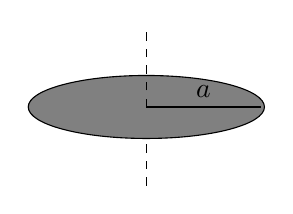
\begin{tikzpicture}
      \draw [fill=gray] circle[x radius = 1.5, y radius = 0.4];
      \draw (0, 0) -- (1.45, 0) node [pos = 0.5, above] {$a$};
      \draw [dashed] (0, -1) -- (0, -0.4);
      \draw [dashed] (0, 0) -- (0, 1);
    \end{tikzpicture}
  \end{center}
  Then
  \begin{align*}
    I &= \int_{0}^{2\pi}\int_0^a \underbrace{\frac{M}{\pi a^2}}_{\text{mass per unit length}} \underbrace{r^2}_{s^2} \underbrace{r\;\d r\;\d \theta}_{\text{area element}}\\
    &= \frac{M}{\pi a^2}\int_0^a r^3\;\d r \int_0^{2\pi}\;\d \theta\\
    &= \frac{M}{\pi a^2}\frac{1}{4}a^4 (2\pi)\\
    &= \frac{1}{2}Ma^2.
  \end{align*}

  Now suppose that the rotation axis is in the plane of the disc instead (also rotating through the center). Then
  \begin{align*}
    I &= \int_{0}^{2\pi}\int_0^a \underbrace{\frac{M}{\pi a^2}}_{\text{mass per unit length}} \underbrace{(r\sin \theta)^2}_{s^2} \underbrace{r\;\d r\;\d \theta}_{\text{area element}}\\
    &= \frac{M}{\pi a^2}\int_0^a r^3\;\d r \int_0^{2\pi}\sin^2 \theta\;\d \theta\\
    &= \frac{M}{\pi a^2}\frac{1}{4}a^4 \pi\\
    &= \frac{1}{4}Ma^2.
  \end{align*}
\end{eg}
\begin{eg}
  Consider a solid sphere with mass $M$, radius $a$, with a rotation axis though the center.
  \begin{center}
    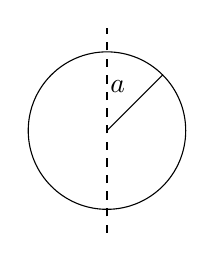
\begin{tikzpicture}
      \draw circle [radius = 1];
      \draw (0, 0) -- (0.707, 0.707) node [pos =0.5, anchor = south east] {$a$};
      \draw [dashed] (0, -1.3) -- (0, 1.3);
    \end{tikzpicture}
  \end{center}
  Using spherical polar coordinates $(r, \theta, \phi)$ based on the rotation axis,
  \begin{align*}
    I &= \int_{0}^{2\pi}\int_0^\pi\int_0^a \underbrace{\frac{M}{\frac{4}{3}\pi a^3}}_{\rho}\underbrace{(r\sin \theta)^2}_{s^2} \underbrace{r^2\sin \theta\;\d r\;\d \theta\;\d \phi}_{\text{volume element}}\\
    &= \frac{M}{\frac{4}{3}\pi a^3}\int_0^a r^4 \;\d r\int_0^\pi (1 - \cos^2)\sin \theta\;\d \theta \int_0^{2\pi}\;\d \phi\\
    &= \frac{M}{\frac{4}{3}\pi a^3}\cdot \frac{1}{5}a^5 \cdot \frac{4}{3}\cdot 2\pi\\
    &= \frac{2}{5}Ma^2.
  \end{align*}
\end{eg}

\begin{thm}[Perpendicular axis theorem]
  For a two-dimensional object (a lamina), and three perpendicular axes $x, y, z$ through the same spot, with $z$ normal to the plane,
  \[
    I_z = I_x + I_y,
  \]
  where $I_z$ is the moment of inertia about the $z$ axis.

  \begin{center}
    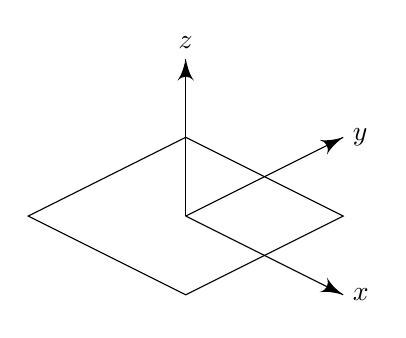
\begin{tikzpicture}
      \draw [->] (0, 0) -- (2, -1) node [right] {$x$};
      \draw [->] (0, 0) -- (2, 1) node [right] {$y$};
      \draw [->] (0, 0) -- (0, 2) node [above] {$z$};
      \draw (-2, 0) -- (0, -1) -- (2, 0) -- (0, 1) -- cycle;
    \end{tikzpicture}
  \end{center}
\end{thm}
\note this does NOT apply to 3D objects! For example, in a sphere, $I_x = I_y = I_z$.

\begin{proof}
  Let $\rho$ be the mass per unit volume. Then
  \begin{align*}
    I_x &= \int \rho y^2 \;\d A\\
    I_Y &= \int \rho x^2 \;\d A\\
    I_z &= \int \rho (x^2 + y^2)\;\d A = I_x + I_y.
  \end{align*}
\end{proof}

\begin{eg}
  For a disc, $I_x = I_y$ by symmetry. So $I_z = 2 I_x$.
\end{eg}

\begin{thm}[Parallel axis theorem]
  If a rigid body of mass $M$ has moment of inertia $I^C$ about an axis passing through the center of mass, then its moment of inertia about a parallel axis a distance $d$ away is
  \[
    I = I^C + Md^2.
  \]
  \begin{center}
    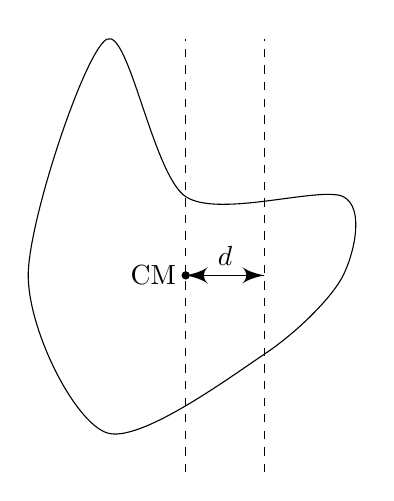
\begin{tikzpicture}
      \draw plot [smooth cycle] coordinates{(0, 0) (1, -2)  (3, -1)  (4, 0)  (4, 1)  (2, 1)  (1, 3)};
      \node [circ] at (2, 0) {};
      \node at (2, 0) [left] {CM};
      \draw [dashed] (2, -2.5) -- (2, 3);
      \draw [dashed] (3, -2.5) -- (3, 3);
      \draw [->] (2, 0) -- (3, 0);
      \draw [->] (3, 0) -- (2, 0) node [pos = 0.5, above] {$d$};
    \end{tikzpicture}
  \end{center}
\end{thm}

\begin{proof}
  With a convenient choice of Cartesian coordinates such that the center of mass is at the origin and the two rotation axes are $x = y =0$ and $x = d, y = 0$,
  \[
    I^C = \int \rho (x^2 + y^2) \;\d V,
  \]
  and
  \[
    \int \rho \mathbf{r}\;\d V = \mathbf{0}.
  \]
  So
  \begin{align*}
    I &= \int \rho((x - d)^2 + y^2)\;\d V\\
    &=\int \rho (x^2 + y^2)\;\d V - 2d\int \rho x\;\d V + d^2 \rho\;\d V\\
    &= I^c + 0 + Md^2\\
    &= I^c + Md^2.
  \end{align*}
\end{proof}

\begin{eg}
  Take a disc of mass $M$ and radius $a$, and rotation axis through a point on the circumference, perpendicular to the plane of the disc. Then
  \begin{center}
    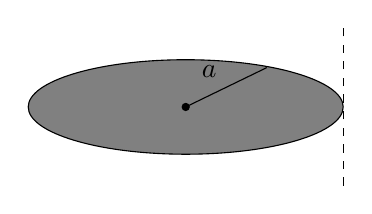
\begin{tikzpicture}
      \draw [fill=gray] circle [x radius = 2, y radius = 0.6];
      \node [circ] {};
      \draw (0, 0) -- (1.03, 0.5) node [pos = 0.5, anchor = south east] {$a$};
      \draw [dashed] (2, -1) -- (2,  1);
    \end{tikzpicture}
  \end{center}
  \[
    I = I^c + Ma^2 = \frac{1}{2}Ma^2 + Ma^2 = \frac{3}{2}Ma^2.
  \]
\end{eg}

\subsection{Motion of a rigid body}
The general motion of a rigid body can be described as a translation of its centre of mass, following a trajectory $\mathbf{R}(t)$, together with a rotation about an axis through the center of mass. We write
\[
  \mathbf{r}_i = \mathbf{R} + \mathbf{r}_i^c.
\]
Then
\[
  \dot{\mathbf{r}}_i = \dot{\mathbf{R}} + \dot{\mathbf{r}}_i^c.
\]
Using this, we can break down the velocity and kinetic energy into translational and rotational parts.

If the body rotates with angular velocity $\boldsymbol\omega$ about the center of mass, then
\[
  \dot{\mathbf{r}}_i^c = \boldsymbol\omega \times \mathbf{r}_i^c.
\]
Since $\mathbf{r}_i^c = \mathbf{r}_i - \mathbf{R}$, we have
\[
  \dot{\mathbf{r}_i} = \dot{\mathbf{R}} + \boldsymbol \omega \times \mathbf{r}_i^c = \dot{\mathbf{r}} + \boldsymbol\omega\times (\mathbf{r}_i - \mathbf{R}).
\]
On the other hand, the kinetic energy (calculated in previous lectures) is
\begin{align*}
  T &= \frac{1}{2}M|\dot{\mathbf{R}}|^2 + \frac{1}{2}\sum_i m_i |\dot{\mathbf{r}}_i^c|^2\\
  &= \underbrace{\frac{1}{2}M|\dot{\mathbf{R}}|^2}_{\text{translational KE}} + \underbrace{\frac{1}{2}I^c\omega^2}_{rotational KE}.
\end{align*}

Sometimes we do not want to use the center of mass as the center. For example, if an item is held at the edge and spun around, we'd like to study the motion about the point at which the item is held, and not the center of mass.

So consider any point $Q$, with position vector $\mathbf{Q}(t)$ that is not the center of mass but moves with the rigid body, ie.
\[
  \dot{\mathbf{Q}} = \dot{\mathbf{R}} + \boldsymbol\omega\times (\mathbf{Q} - \mathbf{R}).
\]
Usually this is a point inside the object itself, but we do not assume that in our calculation.

Then we can write
\begin{align*}
  \dot{\mathbf{r}}_i = \dot{\mathbf{R}} + \boldsymbol\omega\times (\mathbf{r}_i - \mathbf{R})\\
  &= \dot{\mathbf{Q}} - \boldsymbol\omega\times (\mathbf{Q} - \mathbf{R}) + \boldsymbol\omega \times (\mathbf{r}_i - \mathbf{R})\\
  &= \dot{\mathbf{Q}} + \boldsymbol\omega\times (\mathbf{r}_i - \mathbf{Q}).
\end{align*}
Therefore the motion can be considered as a translation of $Q$ (with \emph{different} velocity that the center of mass), together with rotation about $Q$ (with the \emph{same} angular velocity $\boldsymbol\omega$).

\subsubsection*{Equations of motion}
As shown previously, the linear and angular momenta evolve according to
\begin{align*}
  \dot{\mathbf{P}} &= \mathbf{F}\quad \text{(total external force)}\\
  \dot{\mathbf{L}} &= \mathbf{G}\quad \text{(total external torque)}
\end{align*}
These two equations determine the translational and rotational motion of a rigid body. However, in some cases, the conservation is easier to apply.

$\mathbf{L}$ and $\mathbf{G}$ depend on the choice of origin, which could be any point that is fixed in an inertial frame. More surprisingly, it can also be applied to the center of mass, even if this is accelerated:
If
\[
  m_i \ddot{\mathbf{r}}_i = \mathbf{F}_i,
\]
then
\[
  m_i \dot{\mathbf{r}}_i^c = \mathbf{F}_i = m_i \dot{\mathbf{R}}.
\]
So there is a fictitious force in the center-of-mass frame. But the total torque of the fictitious forces about the center of mass is
\[
  \sum_i \mathbf{r}_i^c \times \left(-m_i \ddot{\mathbf{R}}\right) = -\left(\sum m_i \mathbf{r}_i^c\right) \times \ddot{\mathbf{R}} = 0\times \dot{\mathbf{R}} = 0.
\]
So we can still apply the above two equations.

\subsubsection*{Motion in a uniform gravitational field}
In a uniform gravitational field $\mathbf{g}$, the total gravitational force and torque are the same as those that would act on a single particle of mass $M$ located at the center of mass (which is also the \emph{center of gravity}):
\[
  \mathbf{F} = \sum_i \mathbf{F}_i^{\mathrm{ext}} = \sum_i m_i \mathbf{g} = M\mathbf{g},
\]
and
\[
  \mathbf{G} = \sum_i \mathbf{G}_i^{\mathrm{ext}} = \sum_i \mathbf{r}-i \times (m_i \mathbf{g}) = \sum m_i \mathbf{r}_i \times \mathbf{g} = M\mathbf{R}\times \mathbf{g}.
\]
In particular, the gravitational torque about the center of mass vanishes: $\mathbf{G}^c = \mathbf{0}$.

We obtain a similar result for gravitational potential energy.

The gravitational potential in a uniform $\mathbf{g}$ is
\[
  \varphi_g = -\mathbf{r}\cdot \mathbf{g}.
\]
(since $\mathbf{g} = -\nabla \phi_g$ by definition)

So
\begin{align*}
  V^{\mathrm{ext}} &= \sum_i V_i^{\mathrm{ext}}\\
  &= \sum_i m_i (- \mathbf{r}_i \cdot \mathbf{g})\\
  &= M (-\mathbf{R}\cdot \mathbf{g}).
\end{align*}

\begin{eg}[Thrown stick]
  Suppose we throw a symmetrical stick. So the center of mass is the actual center. Then the center of the stick moves in a parabola. Meanwhile, the stick rotates with constant angular velocity about its center due to the absence of torque.
\end{eg}

\begin{eg}
  Swinging bar.
  \begin{center}
    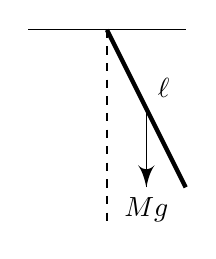
\begin{tikzpicture}
      \draw (-1, 0) -- (1, 0);
      \draw [ultra thick] (0, 0) -- (1, -2) node [anchor = south west, pos = 0.5] {$\ell$};
      \draw [dashed] (0, 0) -- (0, -2.5);
      \draw [->] (0.5, -1) -- (0.5, -2) node [below] {$Mg$};
    \end{tikzpicture}
  \end{center}
  This is an example of a \emph{compound pendulum}.

  Consider the bar to be rotating about the pivot (and not translating). Its angular momentum is $L = I\dot{\theta}$ with $I = \frac{1}{3}m\ell^2$. The gravitational torque about the pivot is
  \[
    G = - Mg\frac{\ell}{2} \sin \theta.
  \]
  The equation of motion is
  \[
    \dot{L} = G.
  \]
  So
  \[
    I\ddot{\theta} = -Mg \frac{\ell}{2}\sin \theta,
  \]
  or
  \[
    \ddot{\theta} = -\frac{3g}{2\ell \sin \theta}.
  \]
  which is exactly equivalent to a simple pendulum of length $2\ell/3$, with angular frequency $\sqrt{\frac{3g}{2\ell}}$.

  This can also be obtained from an energy argument:
  \[
    E = T + V = \frac{1}{2}I\dot{\Theta}^2  - Mg\frac{\ell}{2}\cos\theta.
  \]
  We differentiate to obtain
  \[
    \frac{\d E}{\d t} = \dot{\theta}(I\ddot{\theta} + Mg \frac{\ell}{2}\sin \theta) = 0.
  \]
  So
  \[
    I\ddot{\theta} = -Mg \frac{\ell}{2}\sin \theta.
  \]
\end{eg}

\subsubsection*{Sliding versus rolling}
Consider a cylinder or sphere of radius $a$, moving along a stationary horizontal surface.
\begin{center}
  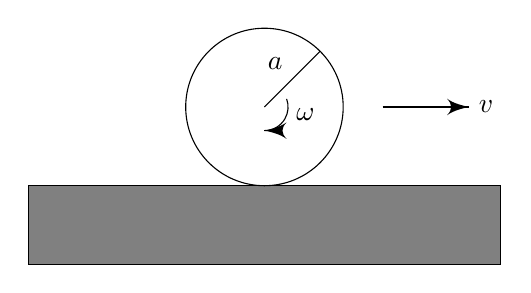
\begin{tikzpicture}
    \draw [fill = gray] (-3, 0) rectangle (3, -1);
    \draw (0, 1) circle [radius=1];
    \draw (0, 1) -- (0.707, 1.707) node [pos=0.5, anchor = south east] {$a$};
    \draw [->] (1.5, 1) -- (2.6, 1) node [right] {$v$};
    \draw (0, 0.7) arc (270:380:0.3) node [anchor = north west] {$\omega$};
    \draw [->] (0.01, 0.7) -- (0, 0.7);
  \end{tikzpicture}
\end{center}

In general, the motion consists of a translation of the center of mass (with velocity $v$) plus a rotation about the center of mass (with angular velocity $\omega$)).

The horizontal velocity at the point of contact is
\[
  v_{\text{slip}} = v - a\omega.
\]
For a pure sliding motion, $v \not = 0$ and $\omega = 0$, in which case $v - a\omega \not = 0$: the point of contact surface and kinetic friction may occur.

For a pure rolling motion, $v\not = 0$ and $\omega \not = 0$ such that $v - a\omega = 0$: the point of contact is stationary: the point of contact is stationary. This is the no-slip condition.

The rolling body can alternatively be considered to be rotating instantaneously about the point of contact (with angular velocity $\omega$) and not translating.

\begin{eg}[Rolling down hill]\leavevmode
  \begin{center}
    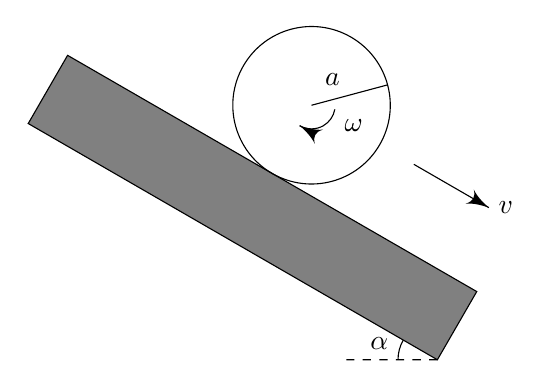
\begin{tikzpicture}[rotate=-30]
      \draw [fill = gray] (-3, 0) rectangle (3, -1);
      \draw (0, 1) circle [radius=1];
      \draw (0, 1) -- (0.707, 1.707) node [pos=0.5, anchor = south east] {$a$};
      \draw [->] (1.5, 1) -- (2.6, 1) node [right] {$v$};
      \draw (0, 0.7) arc (270:380:0.3) node [anchor = north west] {$\omega$};
      \draw [->] (0.01, 0.7) -- (0, 0.7);
      \draw [dashed] (3, -1) -- (2, -1.577);
      \draw (2.5, -1) arc (180:210:0.5) node [anchor = south east] {$\alpha$};
    \end{tikzpicture}
  \end{center}

  Consider a cylinder or sphere of mass $M$ and radius $a$ rolling down a rough plane inclined at angle $\alpha$. The no-slip (rolling) condition is
  \[
    v - a\omega = 0 .
  \]
  The kinetic energy is
  \[
    T = \frac{1}{2}Mv^2 + \frac{1}{2}I\omega^2 = \frac{1}{2}(M + \frac{I}{a^2})v^2.
  \]
  The total energy is
  \[
    E = \frac{1}{2}\left(M + \frac{I}{a^2}\right) \dot{x}^2 - Mgx\sin \alpha,
  \]
  where $x$ is the distance down slope. Energy is conserved (cf. later lectures). So
  \[
    \frac{\d E}{\d t} = \dot{x}\left(\left(M + \frac{I}{a^2}\right)\ddot{x} - Mg\sin \alpha\right) = 0.
  \]
  So
  \[
    \left(M + \frac{I}{a^2}\right)\ddot{x} = Mg\sin \alpha.
  \]
  For example, if we have a uniform solid cylinder,
  \[
    I = \frac{1}{2}Ma^2\quad\text{(as for a disc)}
  \]
  and so
  \[
    \ddot{x} = \frac{2}{3}g\sin \alpha.
  \]
  For a thin cylindrical shell,
  \[
    U = Ma^2.
  \]
  So
  \[
    \ddot{x} = \frac{1}{2}g\sin \alpha.
  \]
  Alternatively, we may do it in terms of forces and torques,
  \begin{center}
    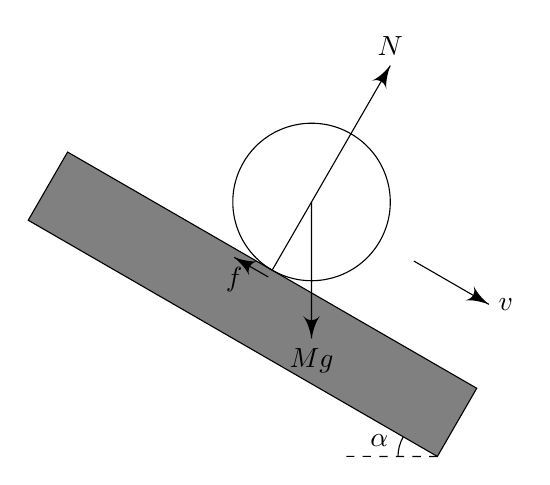
\begin{tikzpicture}[rotate=-30]
      \draw [fill = gray] (-3, 0) rectangle (3, -1);
      \draw (0, 1) circle [radius=1];
      \draw [->] (1.5, 1) -- (2.6, 1) node [right] {$v$};
      \draw [dashed] (3, -1) -- (2, -1.577);
      \draw (2.5, -1) arc (180:210:0.5) node [anchor = south east] {$\alpha$};
      \draw [->] (0, 0) -- (0, 3) node [above] {$N$};
      \draw [->] (0, -0.1) -- (-0.5, -0.1) node [below] {$f$};
      \draw [->] (0, 1) -- (0.866, -0.5) node [below] {$Mg$};
    \end{tikzpicture}
  \end{center}
  The equations of motion are
  \[
    M\dot{v} = Mg\sin \alpha - F
  \]
  and
  \[
    I\dot \omega = aF.
  \]
  While rolling,
  \[
    \dot{v} - a\dot\omega = 0.
  \]
  So
  \[
    M\dot{v} = Mg\sin \alpha - \frac{I}{a^2}\dot{v},
  \]
  leading to the same result.

  Note that even though there is a frictional force, it does no work, since $v_{\mathrm{slip}} = 0$. So energy is still conserved.
\end{eg}

\begin{eg}[Snooker ball]\leavevmode
  \begin{center}
    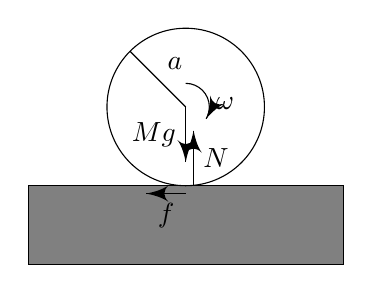
\begin{tikzpicture}
      \draw [fill=gray] (-2, 0) rectangle (2, -1);
      \draw (0, 1) circle [radius=1];
      \draw (0, 1) -- (-0.707, 1.707) node [pos = 0.5, anchor = south west] {$a$};
      \draw [->] (0.1, 0) -- (0.1, 0.7) node [pos = 0.5, right] {$N$};
      \draw [->] (0, 1) -- (0, 0.3)  node [pos = 0.5, left] {$Mg$};
      \draw [->] (0, -0.1) -- (-0.5, -0.1) node [pos = 0.5, below] {$f$};
      \draw [->] (0, 1.3) arc (90:-30:0.3) node [anchor = south west] {$\omega$};
    \end{tikzpicture}
  \end{center}
  It is struck centrally so as to initiate translation, but not rotation. Sliding occurs initially. Intuitively, we think it will start to roll, and we'll see that's the case.

  The constant frictional force is
  \[
    F = \mu_k N = \mu_k Mg,
  \]
  which applies while $v - a\omega > 0$.

  The moment of inertia about the center of mass is
  \[
    I = \frac{2}{5}Ma^2.
  \]
  The equations of motion are
  \begin{align*}
    M\dot{v} &= -F\\
    I\dot\omega &= aF
  \end{align*}
  Initially, $v = v_0$ and $\omega = 0$. Then the solution is
  \begin{align*}
    v &= v_0 - \mu_k gt\\
    \omega &= \frac{5}{2} \frac{\mu_k g}{a}t
  \end{align*}
  as long as $v - a \omega > 0$. The slip velocity is
  \[
    v_{\mathrm{slip}} = v - a\omega = v_0 - \frac{7}{2}\mu_k gt = v_0  \left(1 - \frac{t}{t_\mathrm{roll}}\right),
  \]
  where
  \[
    t_{\mathrm{roll}} = \frac{2v_0}{7\mu_k g}.
  \]
  This is valid up till $t = t_{\mathrm{roll}}$. Then the slip velocity is 0, rolling begins and friction ceases.

  At this point, $v = a\omega = \frac{6}{7}v_0$. The energy is then $\frac{5}{14}Mv_0^2 < \frac{1}{2}Mv_0^2$. So energy is lost to friction.
\end{eg}

\section{Special relativity}
\begin{center}
  \includegraphics[scale=4]{images/xkcd_choices_part_2.jpg}\\
  xkcd (Randall Munroe) CC-BY-NC 2.5
\end{center}
When particles move extremely fast, Newtonian Dynamics becomes inaccurate and is replaced by Einstein's Special Theory of Relativity (1905).

Its effects are noticeable only when particles approach to the speed of light,
\[
  c = \SI{299792458}{\meter\per\second} \approx \SI{3e8}{\meter\per\second}
\]
This \emph{really fast}.

The Special Theory of Relativity rests on the following postulate:

\begin{center}
  \emph{The laws of physics are the same in all inertial frames}
\end{center}

This is the principle of relativity familiar to Galileo. Galilean relativity mentioned in the first chapter satisfies the first postulate for dynamics. People then thought that Galilean relativity is what the world obeys. However, it turns out that there is a whole family of solutions that satisfy the postulate (for dynamics), and Galilean relativity is just one of them.

This is not a problem (yet), since Galilean relativity seems so intuitive, and we might as well take it to be the true one. However, it turns out that solving Maxwell's equations of electromagnetism gives an explicit value of the speed of light, $c$. This is independent of the frame of reference. So the speed of light must be the same in every inertial frame.

This is not compatible with Galilean relativity.

Consider the two inertial frames $S$ and $S'$, related by the Galilean transformation
\[
  x' = x - vt,\quad y' = y,\quad z' = z,\quad t' = t.
\]
In $S$, a light ray (or photon) travels in the $x$ direction at speed $c$. Its trajectory is given by $\frac{x}{t} = c$.

Apply the Galilean transformation. This gives  $\frac{x'}{t'} = \frac{x - vt}{t} = c - v$. So the speed of light in $S'$ would be $c - v$, which is wrong.

Therefore, we need to find a different solution to the principle of relativity that preserves the speed of light.

\subsection{The Lorentz transformation}
Consider again inertial frames $S$ and $S'$ in standard configuration. Assume that the origins of the two frames coincide at $t = t' = 0$. For now, neglect the $y$ and $z$ directions, and consider the relationship between $(x, t)$ and $(x', t')$. The general form is
\[
  x' = f(x, t),\quad t' = g(x, t),
\]
for some functions $f$ and $g$. This is not very helpful.

In any inertial frame, a free particle moves with constant velocity. So straight lines in $(x, t)$ must map into straight liens in $(x', t')$. Therefore the relationship must be \emph{linear}.

Given that the origins of $S$ and $S'$ coincide at $t = t' = 0$, and $S'$ moves with relativity $v$ relative to $S$, we know that the line $x = vt$ must map into $x'= 0$.

Combining these two information, the transformation must be of the form
\[
  x' = \gamma(x - vt),\tag{1}
\]
for some factor $\gamma$ that may depend on $|v|$ (\emph{not} $v$ itself. We can use symmetry arguments to show that $\gamma$ should take the same value for velocities $v$ and $-v$).

Note that Galilean transformation is compatible with this -- just take $\gamma$ to be always $1$.

Now reverse the roles of the frames. From the perspective $S'$, $S$ moves with velocity $-v$. A similar argument leads to
\[
  x = \gamma(x' + vt'),\tag{2}
\]
with the same factor $\gamma$, since $\gamma$ only depends on $|v|$. Now consider a light ray (or photon) passing through the origin $x = x' = 0$ at $t = t' = 0$. Its trajectory in $S$ is
\[
  x = ct.
\]
We want a $\gamma$ such that the trajectory in $S'$ is 
\[
  x' = ct'
\]
as well, so that the speed of light is the same in each frame. Substitute these into (1) and (2)
\begin{align*}
  ct' &= \gamma(c - v)t\\
  ct &= \gamma(c + v)t'
\end{align*}
Multiply the two equations together and divide by $tt'$ to obtain
\[
  c^2 = \gamma^2(c^2 - v^2).
\]
So
\[
  \gamma = \sqrt{\frac{c^2}{c^2 - v^2}} = \frac{1}{\sqrt{1 - (v/c)^2}}.
\]
\begin{defi}[Lorentz factor]
  The \emph{Lorentz factor} is
  \[
    \gamma = \frac{1}{\sqrt{1 - (v/c)^2}}.
  \]
\end{defi}
Note that
\begin{itemize}
  \item $\gamma \geq 1$ and is an increasing function of $|v|$.
  \item When $v \ll c$, then $\gamma \approx 1$, and we recover the Galilean transformation.
  \item When $|v|\to c$, then $\gamma\to \infty$.
  \item If $|V| \geq c$, then $\gamma$ is imaginary, which is physically impossible (or at least \emph{weird}).
  \item If we take $c\to \infty$, then $\gamma = 1$. So Galilean transformation is the transformation we will have if light is infinitely fast. Alternatively, in the world of Special Relativity, the speed of light is ``infinitely fast''.
\end{itemize}
\begin{center}
  \begin{tikzpicture}[xscale=3, yscale=0.2]
    \draw [->] (0, 0) -- (1.1, 0) node [right] {$\frac{v}{c}$};
    \draw [->] (0, 0) -- (0, 15) node [above] {$\gamma$};
    \draw [domain=0:0.997, samples=100] plot (\x, {1 / sqrt(1 - \x * \x)});
    \draw [dashed] (1, 15) -- (1, 0) node [below] {$1$};
  \end{tikzpicture}
\end{center}
For the sense of scale, we have the following values of $\gamma$ at difference speeds:
\begin{itemize}
  \item $\gamma = 2$ when $v = 0.866c$.
  \item $\gamma = 10$ when $v = 0.9965$.
  \item $\gamma = 20$ when $v = 0.999c$.
\end{itemize}

We still have to solve for the relation between $t$ and $t'$. Eliminate $x$ between (1) and (2) to obtain
\[
  x = \gamma(\gamma(x - vt) + vt').
\]
So
\[
  t' = \gamma t - (1 - \gamma^{-2})\frac{\gamma x}{v} = \gamma\left(t - \frac{v}{c^2}x\right).
\]
So we have
\begin{law}[Principle of Special Relativity]
  Let $S$ and $S'$ be inertial frames, moving at the relative velocity of $v$. Then
  \begin{align*}
    x' &= \gamma(x - vt)\\
    t' &= \gamma\left(t - \frac{v}{c^2}x\right),
  \end{align*}
  where
  \[
    \gamma = \frac{1}{\sqrt{1 - (v/c)^2}}.
  \]
  This is the \emph{Lorentz transformations} in the standard configuration (in one spatial dimension).
\end{law}
We can invert this linear mapping to find (after some algebra)
\begin{align*}
  x &= \gamma(x' + vt')\\
  t &= \gamma\left(t' + \frac{v}{c^2}x'\right)
\end{align*}
Directions perpendicular to the relative motion of the frames are unaffected:
\begin{align*}
  y' &= y\\
  z' &= z
\end{align*}
Historical side note: Why is it the \emph{Lorentz transform} but \emph{Einstein}'s theory of relativity? Long story short, Lorentz came up with the equations, and said that ``these weird equations seem to work''. Then Einstein came and said ``because that's what the world actually is!''.\footnote{To be fair, Einstein came up with a lot of the important implications of the Lorentz transformations, including the infamous $E =mc^2$.}

Now we check that the speed of light is really invariant:

For a light ray travelling in the $x$ direction in $S$:
\[
  x = ct,\quad y = 0,\quad z = 0.
\]
In $S'$, we have
\[
  \frac{x'}{t'}\frac{\gamma(x - vt)}{\gamma(t - vx/c^2)} = \frac{(c - v)t}{(1 - v/c)t} = c,
\]
as required.

For a light ray travelling in the $Y$ direction in $S$,
\[
  x = 0,\quad y = ct,\quad z = 0.
\]]
In $S'$,
\[
  \frac{x'}{t'} = \frac{\gamma(x - vt)}{\gamma(t - vx/c^2)} = -v,
\]
and
\[
  \frac{y'}{t'} = \frac{y}{\gamma(t - vx/c^2} = \frac{c}{\gamma},
\]
and
\[
  z' = 0.
\]
So the speed of light is
\[
  \frac{\sqrt{x'^2 + y'^2}}{t'} = \sqrt{v^2 + \gamma^{-2}c^2} = c,
\]
as required.

More generally, the Lorentz transformation implies
\begin{align*}
  c^2t'^2 - r'^2 &= c^2t'^2 - x'^2 - y'^2 - z'^2\\
  &= c^2 \gamma^2\left(t - \frac{v}{c^2}x\right)^2 - \gamma^2(x - vt)^2 - y^2 - z^2\\
  &= \gamma^2\left(1 - \frac{v^2}{c^2}\right)(c^2t^2 - x^2) - y^2 - z^2\\
  &= c^2t^2 - x^2 - y^2 - z^2\\
  &= c^2t^2 - r^2.
\end{align*}
We say that the quantity $c^2t^2 - x^2 - y^2 - z^2$ is \emph{Lorentz-invariant}.

So if $\frac{r}{t} = c$, then $\frac{r'}{t'} = c$ also.

\subsection{Spacetime diagrams}
When considering one spatial dimension $x$ and time $t$ in an inertial frame $S$, we plot $x$ on the horizontal axis and $ct$ on the vertical axis. We use $ct$ instead of $x$ so that the dimensions make sense.

\begin{center}
  \begin{tikzpicture}[yscale=1.3]
    \draw [->] (0, 0) -- (3, 0) node [right] {$x$};
    \draw [->] (0, 0) -- (0, 2.3) node [above] {$ct$};
    \draw (0.7, 0.3) .. controls (0.7, 0.8) and (2, 1.3) .. (2, 1.8) node [right] {world line};

    \node [circ] at (1.35, 1.05) {};
    \node at (1.35, 1.05) [anchor = north west] {$P$};
  \end{tikzpicture}
\end{center}
\begin{defi}[Spacetime]
  The union of space and time in special relativity is called \emph{Minkowski spacetime}. Each point $P$ represents an \emph{event}, labelled by coordinates $(ct, x)$ (note the order!).

  A particle traces out a \emph{world line} in spacetime, which is straight if the particle moves uniformly.

  Light rays moving in the $x$ direction have world lines inclined at $25^\circ$.
  \begin{center}
    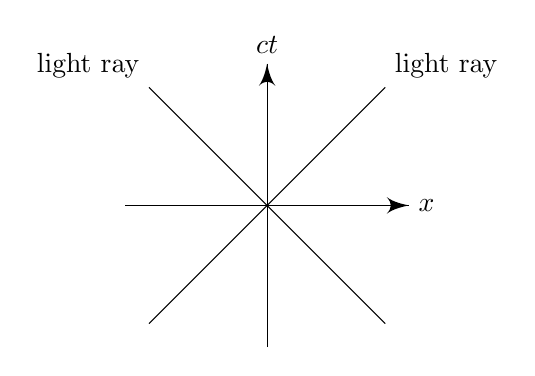
\begin{tikzpicture}[scale=0.6]
      \draw [->] (-3, 0) -- (3, 0) node [right] {$x$};
      \draw [->] (0, -3) -- (0, 3) node [above] {$ct$};
      \draw (-2.5, -2.5) -- (2.5, 2.5) node [anchor = south west] {light ray};
      \draw (2.5, -2.5) -- (-2.5, 2.5) node [anchor = south east] {light ray};
    \end{tikzpicture}
  \end{center}
\end{defi}

We can also draw the axes of $S'$, moving in the $x$ direction at velocity $v$ relative to $S$. The $ct'$ axis corresponds to $x' = 0$, ie. $x = \frac{v}{c}(ct)$. The $x'$ axis corresponds to $t' = 0$, ie. $ct = \frac{v}{c}x$.
\begin{center}
  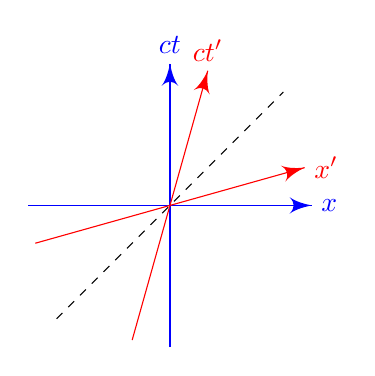
\begin{tikzpicture}[scale=0.6]
    \draw [->, blue] (-3, 0) -- (3, 0) node [right] {$x$};
    \draw [->, blue] (0, -3) -- (0, 3) node [above] {$ct$};
    \draw [->, red] (-2.85, -0.8) -- (2.85, 0.8) node [right] {$x'$};
    \draw [->, red] (-0.8, -2.85) -- (0.8, 2.85) node [above] {$ct'$};
    \draw [dashed] (-2.4, -2.4) -- (2.4, 2.4);
  \end{tikzpicture}
\end{center}
Note that the $x'$ and $ct'$ axes are \emph{not} orthogonal, but are symmetrical about the diagonal (dashed line). So they agree on where the world line of a light ray should lie on.
\subsection{Relativistic physics}
\subsubsection*{Simultaneity}
\begin{defi}[Simultaneous events]
  We say two events $P_1$ and $P_2$ are simultaneous in the frame $S$ if $t_1 = t_2$.
\end{defi}
They are represented in the following spacetime diagram by horizontal dashed lines.

However, events that are simultaneous in $S'$ have equal values of $t'$, and sol lie on lines
\[
  ct - \frac{v}{c}x = \text{constant}.
\]

\begin{center}
  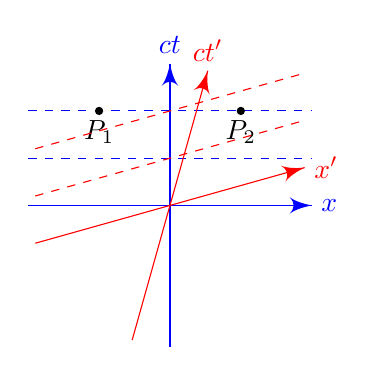
\begin{tikzpicture}[scale=0.6]
    \draw [->, blue] (-3, 0) -- (3, 0) node [right] {$x$};
    \draw [->, blue] (0, -3) -- (0, 3) node [above] {$ct$};
    \draw [dashed, blue] (-3, 1) -- (3, 1);
    \draw [dashed, blue] (-3, 2) -- (3, 2);
    \node [circ] at (-1.5, 2) {};
    \node [circ] at (1.5, 2) {};
    \node at (-1.5, 2) [below] {$P_1$};
    \node at (1.5, 2) [below] {$P_2$};
    \draw [->, red] (-2.85, -0.8) -- (2.85, 0.8) node [right] {$x'$};
    \draw [dashed, red] (-2.85, 0.2) -- (2.85, 1.8);
    \draw [dashed, red] (-2.85, 1.2) -- (2.85, 2.8);
    \draw [->, red] (-0.8, -2.85) -- (0.8, 2.85) node [above] {$ct'$};
  \end{tikzpicture}
\end{center}
The lines of simultaneity of $S'$ and those of $S$ are different, and events simultaneous in $S$ need not be simultaneous in $S'$. So simultaneity is relative. $S$ thinks $P_1$ and $P_2$ happened at the same time, while $S'$ thinks $P_2$ happens first.

Note that this is genuine disagreement. It is not due to effects like, it takes time for the light conveying the information to different observers. Our account above already takes that into account! (by not mentioning the existence of an observer :)

\subsubsection*{Causality}
Although different people may disagree on the temporal order of events, the consistent ordering of cause and effect can be ensured.

Since things can only travel at at most the speed of light, $P$ cannot affect $R$ if $R$ happens a millisecond after $P$ but is at millions of galaxies away. We can draw a \emph{light cone} that denotes the regions in which things can be influenced by $P$. These are the regions of space-time light (or any other particle) can possibly travel to. $P$ can only influence events within its \emph{future light cone}, and \emph{be} influenced by events within its \emph{past light cone}.

\begin{center}
  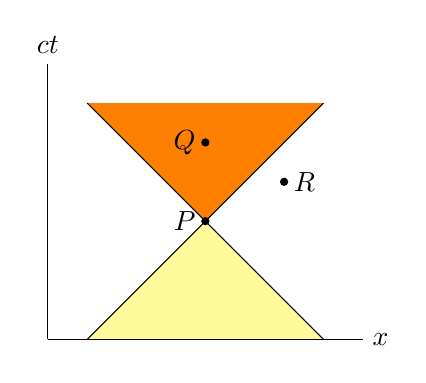
\begin{tikzpicture}
    \draw [fill=white!60!yellow] (0.5, 0) -- (2, 1.5) -- (3.5, 0);
    \draw [fill=red!50!yellow] (0.5, 3) -- (2, 1.5) -- (3.5, 3);
    \draw (0, 0) -- (4, 0) node [right] {$x$};
    \draw (0, 0) -- (0, 3.5) node [above] {$ct$};
    \node [circ] at (2, 1.5) {};
    \node at (2, 1.5) [left] {$P$};
    \node [circ] at (2, 2.5){};
    \node at (2, 2.5) [left] {$Q$};
    \node [circ] at (3, 2) {};
    \node at (3, 2) [right] {$R$};
  \end{tikzpicture}
\end{center}

All observers agree that $Q$ occurs after $P$. Different observers may disagree on the temporal ordering of $P$ and $R$. However, since nothing can travel faster than light, $P$ and $R$ cannot influence each other. Since everyone agrees on how fast light travels, they also agree on the light cones, and hence causality. So philosophers are happy.
\end{document}
